\begin{savequote}[75mm]
Passion is in all great searches and is necessary to all creative endeavors.
\qauthor{W. Eugene Smith}
\end{savequote}

\chapter{Search for Higgs pair production in boosted $\FourB$ final states}
\label{chap:boosted4b}

\section{Introduction}

After the discovery of the Higgs boson in the ATLAS Run 1 dataset and the subsequent measurements of its properties, the Higgs transformed into a potential tool in searches for physics beyond the Standard Model. The pair production cross section of the Higgs can be enhanced through BSM physics. Studying di-Higgs production also probes the Higgs self-coupling, shedding light on the structure of the Higgs potential. This chapter presents a search for resonant production of a Higgs pair in the $\FourBfull$ final state in $3.2 \ifb$ of data collected at $\sqrt{s} = 13 \TeV$. In particular, this chapter focuses on a search for this final state in the regime where $m_{X}$ is large ($\gtrsim 1 \TeV$) and the Higgs bosons in the decay are significantly boosted. A tailored selection for this boosted selection, using novel techniques in jet substructure and $b$-tagging, is discussed. Then, the data-driven background estimate is presented. Finally, the results of the search are shown. The signal models used as benchmarks are a spin-$2$ Rnadall Sundrum graviton (RSG) and a narrow width spin-$0$ resonance. These models are described in more detail in Chapter 1. Limits on signal models are reserved for the next chapter where the results of this chapter are combined with the results of a separate selection dedicated to the lower $m_X$ regime. 

\section{Motivation}

With the center of mass energy increase from $\sqrt{s} = 8 \TeV$ to $\sqrt{s} = 13 \TeV$, the LHC and ATLAS are able to probe new resonances at higher mass scales than previously accessible in Run 1. This is a powerful motivator for searching for a new resonance in the early $13 \TeV$ data. Figure~\ref{fig:lumi_ratio} shows the ratios of parton luminosities between $8$ and $13 \TeV$ for different resonance masses. For a resonance of $M_{X} = 2 \TeV$, the cross section at $\sqrt{s} = 13 \TeV$ is roughly a factor of $10$ larger than at $\sqrt{s} = 8 \TeV$. 

\begin{figure}[h!]
  %\vspace{20pt}
  \centering
  \captionsetup{justification=centering}

  %\hspace*{-32pt}
  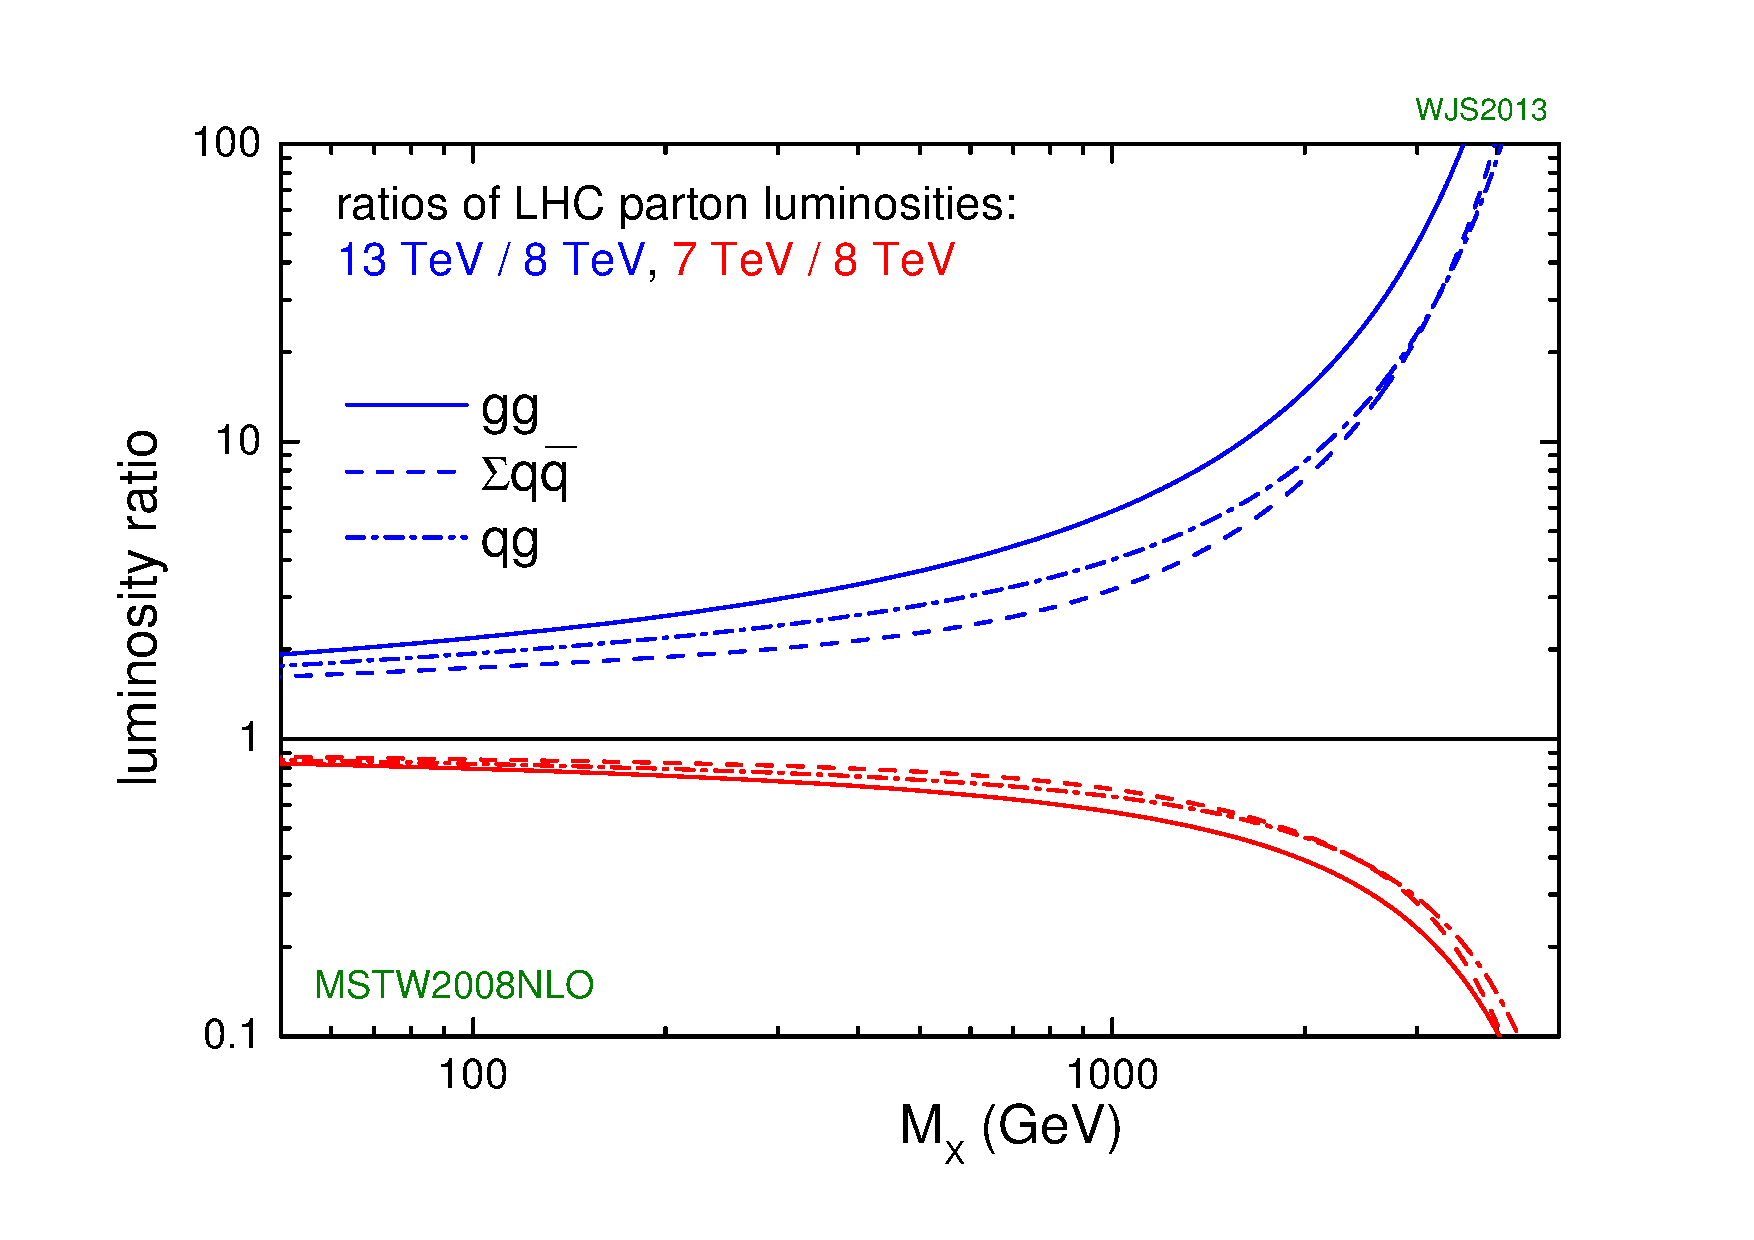
\includegraphics[width=0.6\textwidth,angle=270]{figures/Stirling_lumi_ratios}
  \caption{Parton luminosity ratios as a function of resonance mass $M_{X}$ for $13/8 \TeV$ and $7/8 \TeV$~\cite{LumiRatio}.}
  \label{fig:lumi_ratio}
\end{figure}

Higgs pair production offers a vast array of unprobed regions of phase space where searches for BSM physics can be made. Chapter 1 discusses some possibilities for both resonant and non-resonant enhancement of the di-Higgs production cross section. Given the increased mass reach of the LHC in Run 2, it is particularly important to focus on resonant searches at high $m_{X}$. One consideration when conducting a search in the $HH$ final state is which decay modes of the Higgs to consider. Figure~\ref{fig:HH_BR} shows the branching ratio of the $HH$ final state for different combinations of decays of each individual Higgs. As the largest branching ratio for the $125 \GeV$ Higgs is $H\to b\bar{b}$, the $HH\to b\bar{b}b\bar{b}$ branching ratio is also the largest at $33\%$. 

\begin{figure}[h!]
  %\vspace{20pt}
  \centering
  \captionsetup{justification=centering}

  %\hspace*{-32pt}
  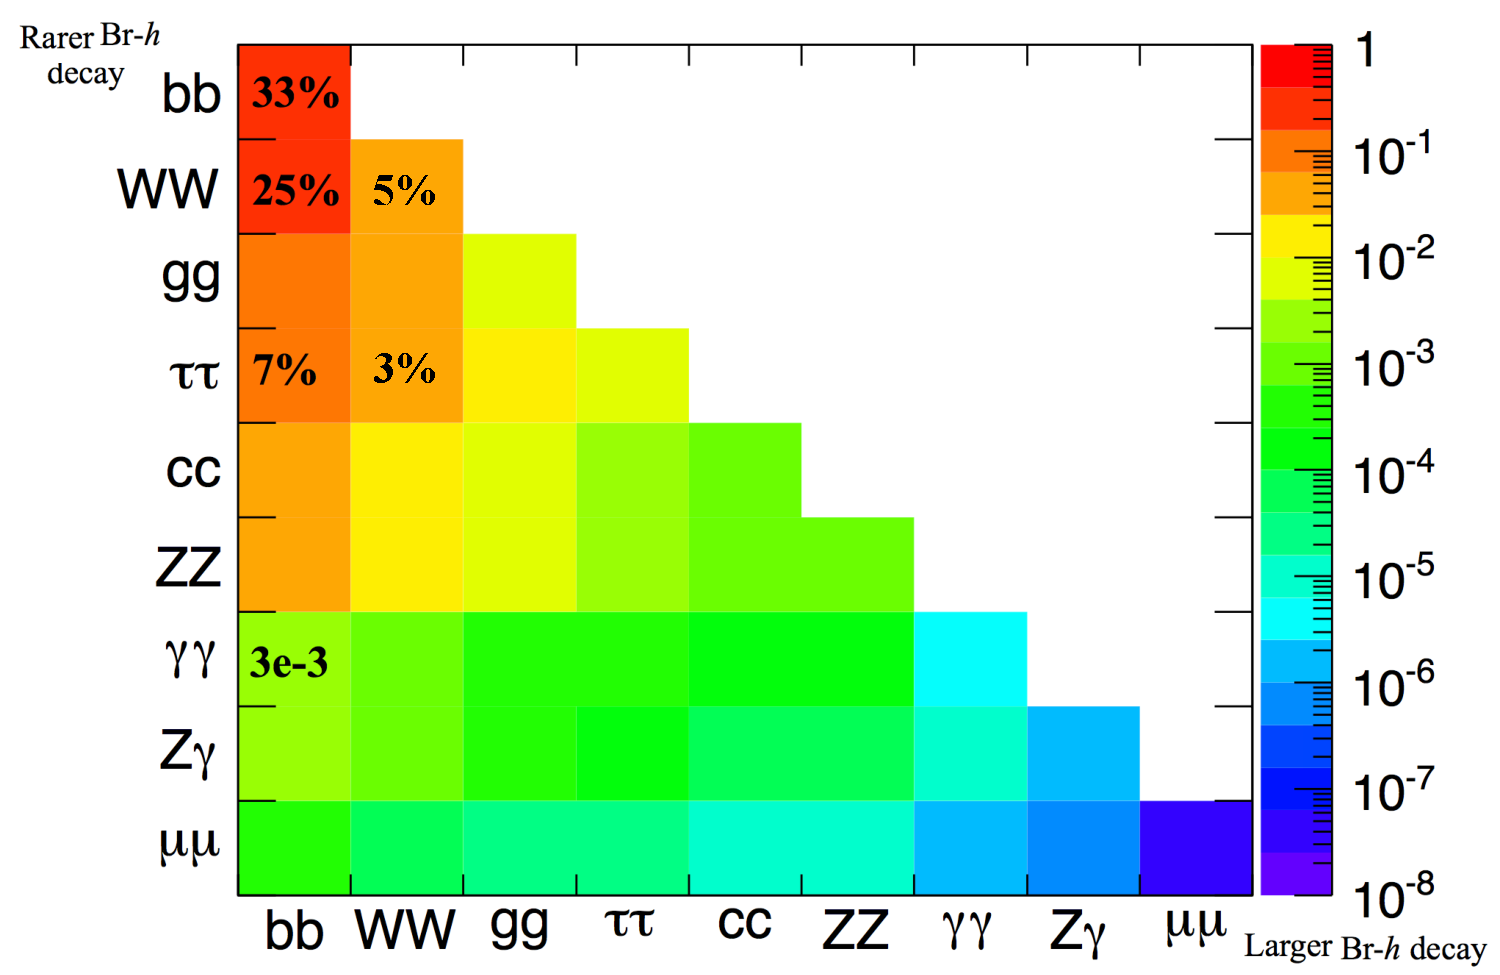
\includegraphics[width=0.8\textwidth]{figures/HH_BR}
  \caption{Summary of $HH$ branching ratios~\cite{HH_BR}.}
  \label{fig:HH_BR}
\end{figure}

At high $m_{X}$, the Higgs bosons resulting from the decay of a heavy resonance will have large $\pT$\footnote{In the limit that $m_{H} \ll m_{X}$, the Higgs $\pT$ is roughly $m_{X}/2$.}. The $\Delta R$ between the decay products of the Higgs is inversely proportional to the Higgs $\pT$, as shown in equation~\ref{eqn:bb_dr}. 

\begin{equation}
\Delta R \approx \frac{2m}{\pT}
\end{equation}

Figure~\ref{fig:bb_dr} shows the minimum $\Delta R$ between truth level $B$ decay vertices in simulation samples for Randall-Sundrum gravitons of different masses. The figure shows that as the mass of the graviton increases, the $\Delta R$ distribution between the $b$ quarks in the Higgs decay tends to shift to lower values. Because of this effect, it is necessary to tailor a selection to target these merged $b$-jets. 

\begin{figure}[h!]
  %\vspace{20pt}
  \centering
  \captionsetup{justification=centering}

  %\hspace*{-32pt}
  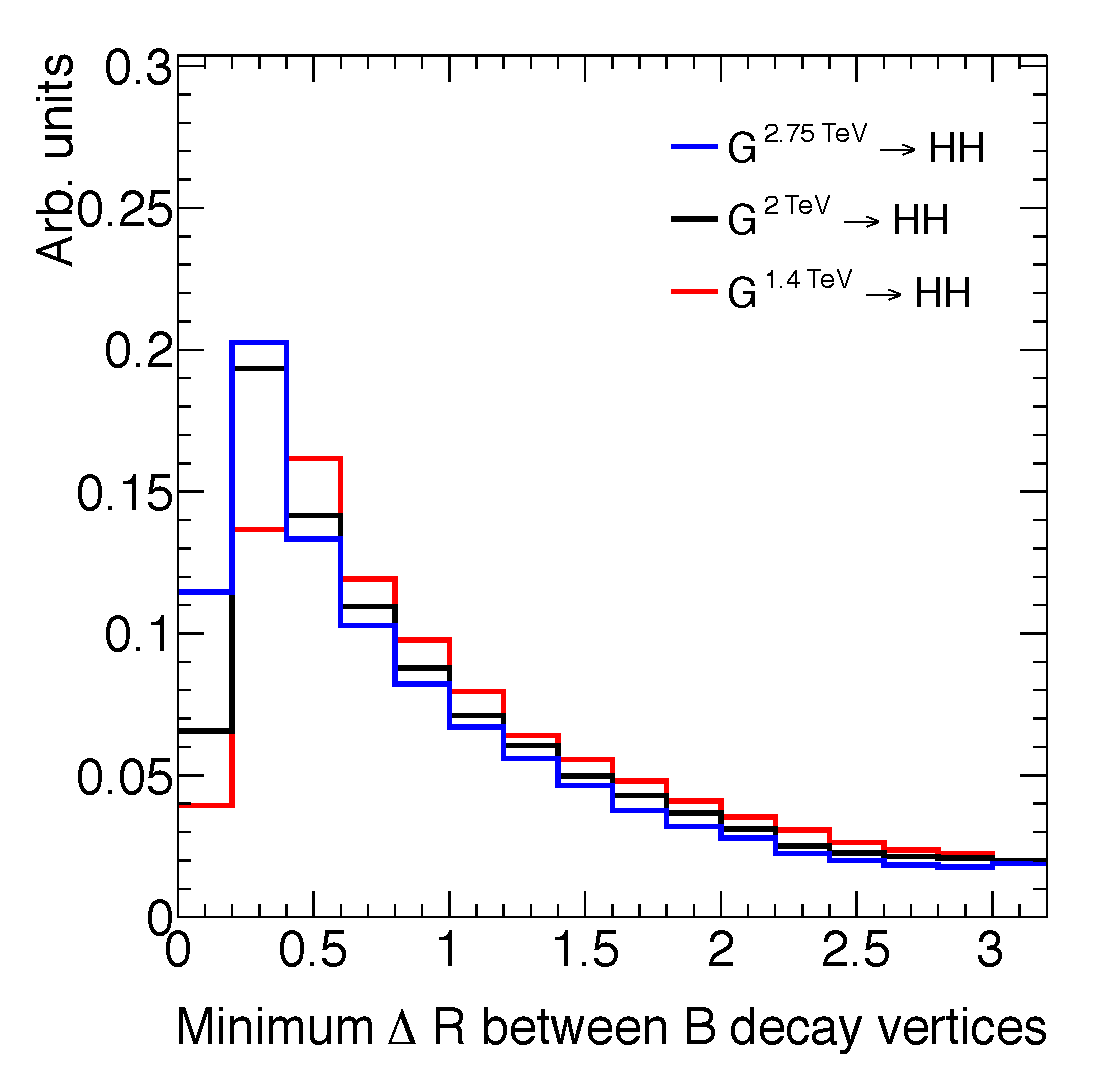
\includegraphics[width=0.5\textwidth]{figures/min_dR_bb}
  \caption{Minimum $\Delta R$ between $B$ decay vertices for different RSG masses in a $\Gkk \to HH \to 4b$ sample with $c = 1$}
  \label{fig:bb_dr}
\end{figure}

\section{Data and simulation samples}

\subsection{Signal models}

While the resonance search is by its nature generic (as it is a simple search for a peak in the $4b$ invariant mass spectrum), there are two signal models that the selection requirements have been optimized for. The first is  Randall-Sundrum (RSG) model, where a tower of massive spin-$2$ Kaluza-Klein gravitons is predicted. The second is a heavy narrow spin-$0$ resonance, the so-called ``heavy Higgs". This type of resonance arises, for example, in the two Higgs doublet model (2HDM). More details about the physics of these models and their motivation is given in chapter 1. 

Signal graviton ($\Gkk$) events are generated at leading order (LO) with \MADGRAPH 5 v$2.2.2$~\cite{MG5aMCatNLO}. The PDF set used is the \NNPDF 2.3 LO set~\cite{nnpdf}. For modeling parton shower and hadronization in jets, \PYTHIA $8.186$ is used with the A$14$ tune~\cite{pythia8,a14tune}. The free parameters in the RSG model are the graviton mass and the coupling constant $c \equiv k/\bar{M}_{\rm Pl}$\footnote{$k$ is the curvature constant for the warped extra dimension and $\bar{M}_{\rm Pl}$ is the Planck mass divided by $8\pi$}. Both the production cross section and width of the graviton are proportional to $c^2$. Samples are generated at both $c = 1$ and $c = 2$ for a variety of mass points between $300 \GeV$ and $3 \TeV$. 

The second signal sample is a heavy spin-$0$ resonance $H$ with a fixed width of $\Gamma_H = 1 \GeV$. This is generated with \MADGRAPH 5 and uses the \CT10 PDF set~\cite{ct10}. The parton shower and hadronization are handled by \HERWIG++ with the \CTEQ6L1 PDF set and the UEEE5 event tune~\cite{HerwigPP,cteq,UEEE5}. Because the width and branching ratios depend on 2HDM parameters, each mass point generated with this fixed width corresponds to a different point in the 2HDM parameter phase space. Mass points are generated between $300 \GeV$ and $1 \TeV$ as with the RSG signal samples. 

\subsection{Background samples}

While the dominant QCD multijet background is estimated with a fully data-driven method, the sub-dominant backgrounds $t\bar{t}$ and $Z$+jets are modeled with some input from simulation.

$\ttbar$ events are simulated at next-to-leading order (NLO) with the \POWHEGBOX version 1 generator using the \CT10 PDF set~\cite{PowhegBox}. The parton shower, hadronization, and underlying event are simulated with \PYTHIA 6.428 with the \CTEQ6L1 PDF set~\cite{pythia6}. The Perugia 2012 tune is used~\cite{Perugia2012}. NNLO QCD corrections to the cross sections are computed in Top++ 2.0~\cite{TopPP}. The top quark mass is set to $172.5 \GeV$. The shapes of distributions in $\ttbar$ are taken from MC while the normalization is taken from data.

Finally, the $Z$+jets background is simulated with \PYTHIA $8.186$ and the \NNPDF 2.3 LO PDF set. This background is negligible compared to the others and is taken fully from MC. 

\subsection{Data sample and trigger}

This analysis is done on $3.2 \ifb$ of data taken in $2015$ at $\sqrt{s} = 13 \TeV$. The details of the machine conditions during this time can be found in Chapter 2. Only data which was taken during stable beam conditions with all detectors functioning is used. Events must pass a trigger which requires a single $360 \GeV$ large radius ($R=1.0$) jet to be reconstructed in the HLT. Figure~\ref{fig:trig_eff_4b} shows the trigger efficiency for various trigger options as a function of graviton mass. Above $m_{G} > 1 \TeV$, the single large radius jet trigger is $99\%$ efficient for events passing the signal selection. 

\begin{figure}[h!]
  %\vspace{20pt}
  \centering
  \captionsetup{justification=centering}

  %\hspace*{-32pt}
  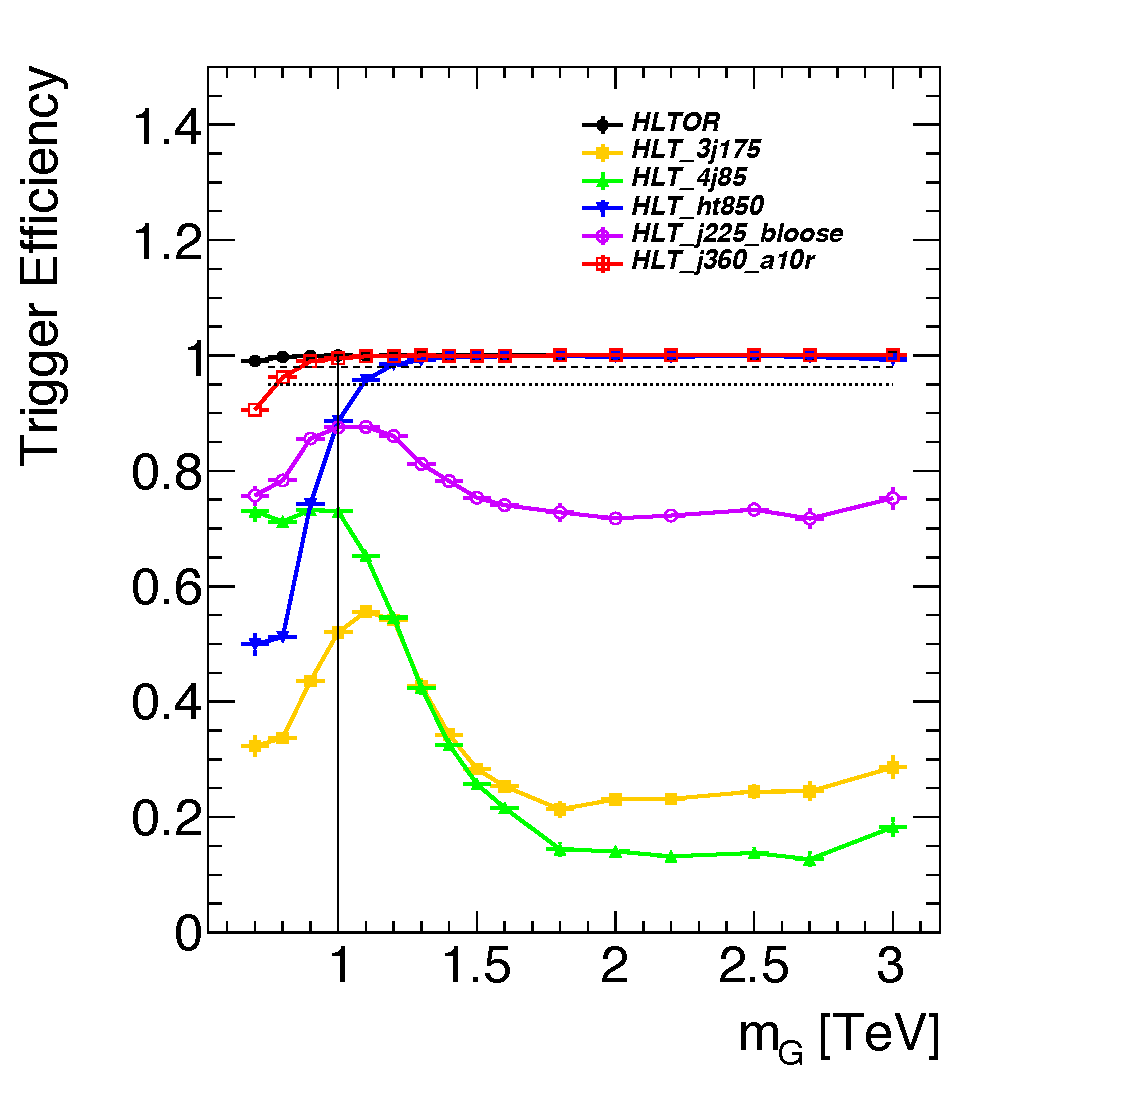
\includegraphics[width=0.7\textwidth]{figures/PassSignal_HLTeff}
  \caption{Trigger efficiency for events passing all signal region selections as a function of mass in $\Gkk \to HH \to 4b$ samples with $c = 1$~\cite{Tony}. In the trigger names, ``j" refers to a jet or jets. ``ht" refers to $H_{T}$, the scalar sum of transverse momenta in the event. ``bloose" refers to a loose $b$-tagging requirement applied to the jet. ``a10r" refers to anti-$k_{T}$ jets with $R = 1.0$. The numbers at the end are the thresholds on the given quantity in $\GeV$.}
  \label{fig:trig_eff_4b}
\end{figure}

\section{Event reconstruction and object selection}

The boosted selection first begins by defining a unique set of objects that can be exploited to increase signal efficiency in the kinematic regime where the final state $b$-jets are very merged. 

\subsection{Large radius ($R = 1.0$)\, jets}

The first step towards reconstructing the final state is to define objects that can be used to measure the kinematics of the Higgs bosons. In the boosted selection anti-$k_{T}$ jets with a radius parameter of $1.0$ are used. These jets is much larger in angular size than the typical $R=0.4$ jets and are intended to encompass both jets resulting from the Higgs decay\footnote{This is in contrast to the resolved selection, which uses two $R=0.4$ anti-$k_{T}$ jets for each Higgs}. The jets are built from clusters in the calorimeter calibrated with local calibration weighting~\cite{JetCalib}. 

Because of the large extent of these jets, great care must be taken to remove potential contrubutions of calorimeter clusters from pile-up. This is done using a technique called jet trimming~\cite{Trimming}. With trimming, the constituents of the large radius jet are re-clustered with a smaller radius with the $k_{T}$ algorithm. Then, these so-called subjets are removed from the larger jet if $p_{T}^{\rm subjet}/p_{T}^{\rm jet} < f_{\rm cut}$. In this analysis, the subjet radius is $R = 0.2$ and $f_{\rm cut} = 0.05$. Trimming has been shown to improve the mass resolution of large radius jets. Figure~\ref{fig:trimming} shows the effect of trimming on the large radius jet mass ($\MJ$). Because the large radius jet fully contains the higgs decay products, its invariant mass should correspond to the $125 \GeV$ mass of the Higgs. The trimming algorithm brings the jet mass much closer to the expected Higgs mass and improves the mass resolution. 

\begin{figure}[h!]
  %\vspace{20pt}
  \centering
  \captionsetup{justification=centering}

  %\hspace*{-32pt}
  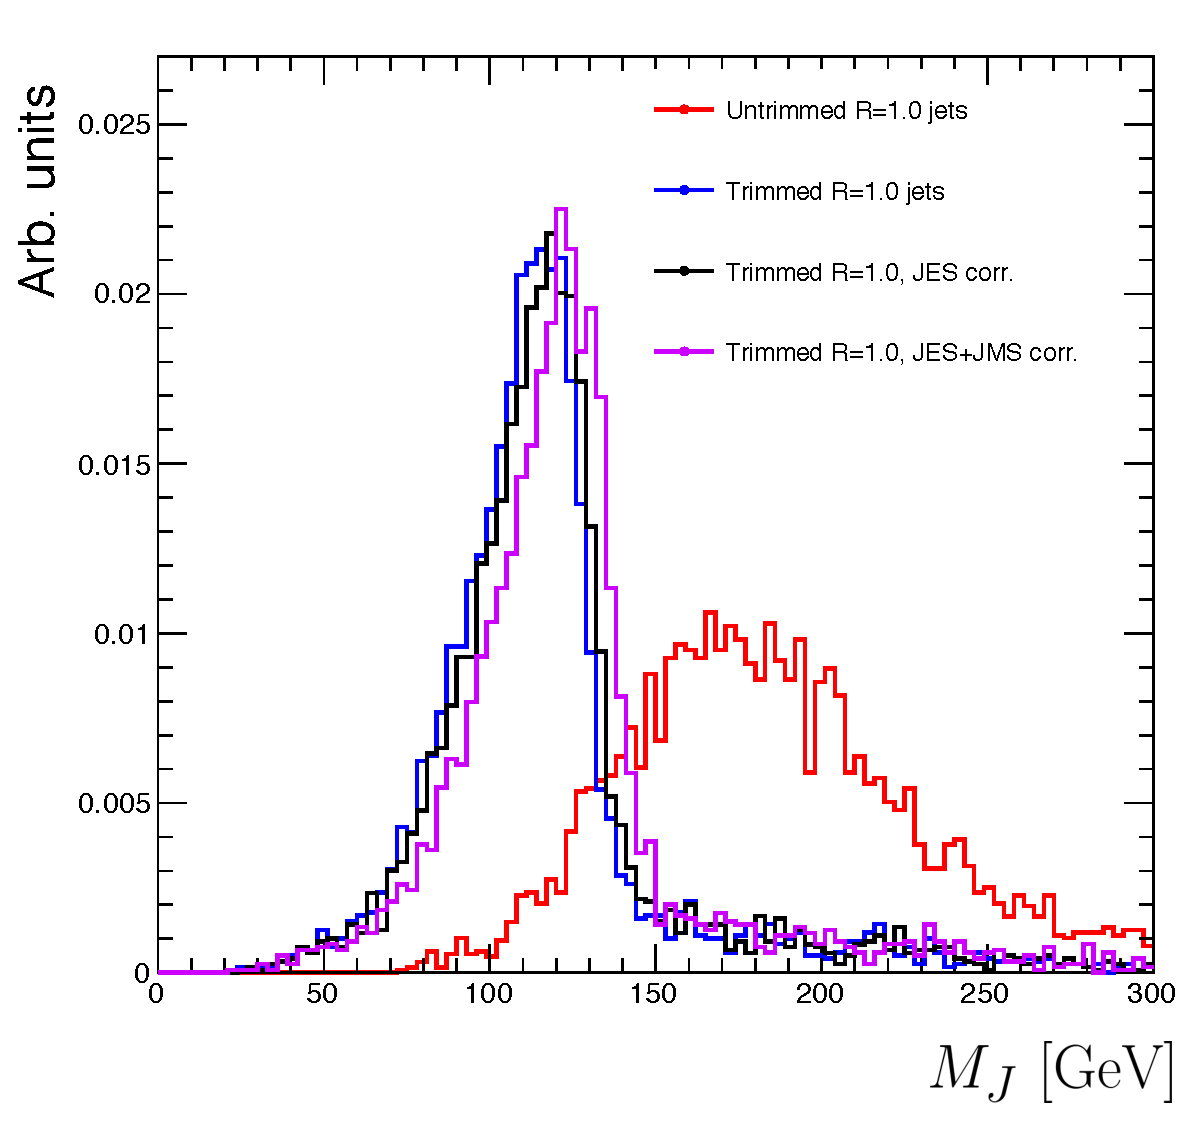
\includegraphics[width=0.6\textwidth]{figures/Trimmed_Mass}
  \caption{Comparison of untrimmed and trimmed jet masses for large radius jets in a RSG sample with $m_{\Gkk} = 1 \TeV$. JES (JMS) refers to the standard jet energy (mass) scale calibration for ATLAS~\cite{JetCalib}.}
  \label{fig:trimming}
\end{figure}

The large radius jets are required to satisfy $250 < \pt < 1500 \GeV$.  They must also be within $|\eta| < 2.0$ in order to ensure that the full jet is within the inner detector tracking volume. Finally, they are required to have $\MJ > 50 \GeV$. The upper $\pT$ cut and lower threshold on mass are applied to correspond to the kinematic range where uncertainties are available in ATLAS calibrations~\cite{BoostedW,BoostedHiggs}.

\subsection{Track jets and $b$-tagging}

Because the $b$-jets from boosted Higgs decays are so close together (as illustrated in figure~\ref{fig:bb_dr}), narrow radius jets are required to fully resolve both $b$-jets. The minimum radius feasible for jets based on calorimeter deposits is determined by the calorimeter granularity. However, because $b$-tagging relies on information from the inner detector, it is possible to define another type of jet that can have a smaller radius and better $b$-tagging resolution. These jets are called ``track jets"~\cite{TrackJets,BoostedHiggs}.

Track jets are formed by applying the usual anti-$k_{T}$ clustering algorithm to tracks that are required to be consistent with the primary vertex. After the jet axis has been determined using these tracks, a second step of track association is also performed to add tracks that can be useful for $b$-tagging~\cite{TrackJets}. In this analysis, the tracks are clustered with a radius parameter of $R = 0.2$. This radius has been shown to give good performance in boosted Higgs tagging~\cite{TrackJets,BoostedHiggs}. Figure~\ref{fig:rcomp} shows a comparison among different track jet radii of the efficiency for reconstructing two $b$-jets from each Higgs in a RSG sample as a function of mass. Track jets with radius of $0.2$ give the best performance, especially at high mass. 

\begin{figure}[h!]
  %\vspace{20pt}
  \centering
  \captionsetup{justification=centering}

  %\hspace*{-32pt}
  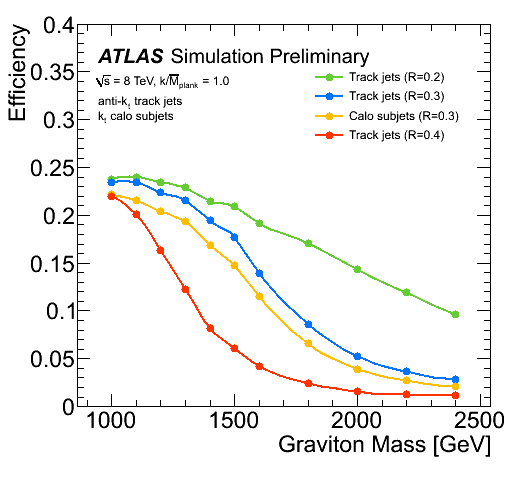
\includegraphics[width=0.6\textwidth]{figures/TrackJet_RComp}
  \caption{Efficiency of finding two $b$-jets from each Higgs in an RSG event using calorimeter jets with $R=0.3$ or different track jet radii~\cite{TrackJets}}
  \label{fig:rcomp}
\end{figure}

In this analysis, track jets are required to have $p_{T} > 10 \GeV$ and $|\eta| < 2.5$. They must also have at least two tracks. 

\subsection{Muons}

Muons are used in this study to correct the four-momenta of calorimeter jets by accounting for semi-leptonic $b$ decays. The muons used are combined ID and MS muons which must satisfy tight identification requirements~\cite{MuonReco}. The muons must have $\pT > 4 \GeV$ and $|\eta| < 2.5$. Table~\ref{tab:4b_req} summarizes the object requirements described in this section.

\begin{table}[h!]
\centering
\captionsetup{justification=centering}

%\begin{tabular*}{0.480\textwidth}{p{0.075\textwidth} p{0.180\textwidth} l}
\hspace{-10pt}
\begin{tabular}{|c|c|c|c|c|}
\hline
& $R$ & $\pT $ & $|\eta|$ & $M$ \\ \hline
Calorimeter jets & $1.0$ & $250 < \pT < 1500 \GeV$ & $ < 2.0$ & $ > 50 \GeV$ \\ \hline
Track jets & $0.2$ & $> 10 \GeV$ & $< 2.5$ & - \\ \hline
Muons & - & $4 \GeV$ & $< 2.5$ & - \\ \hline
\end{tabular}

\caption{
Summary of requirements on objects used in the $\FourBfull$ search
}
\label{tab:4b_req}
\end{table}

\section{Event selection}

\begin{figure}[h!]
  %\vspace{20pt}
  \centering
  \captionsetup{justification=centering}

  %\hspace*{-32pt}
  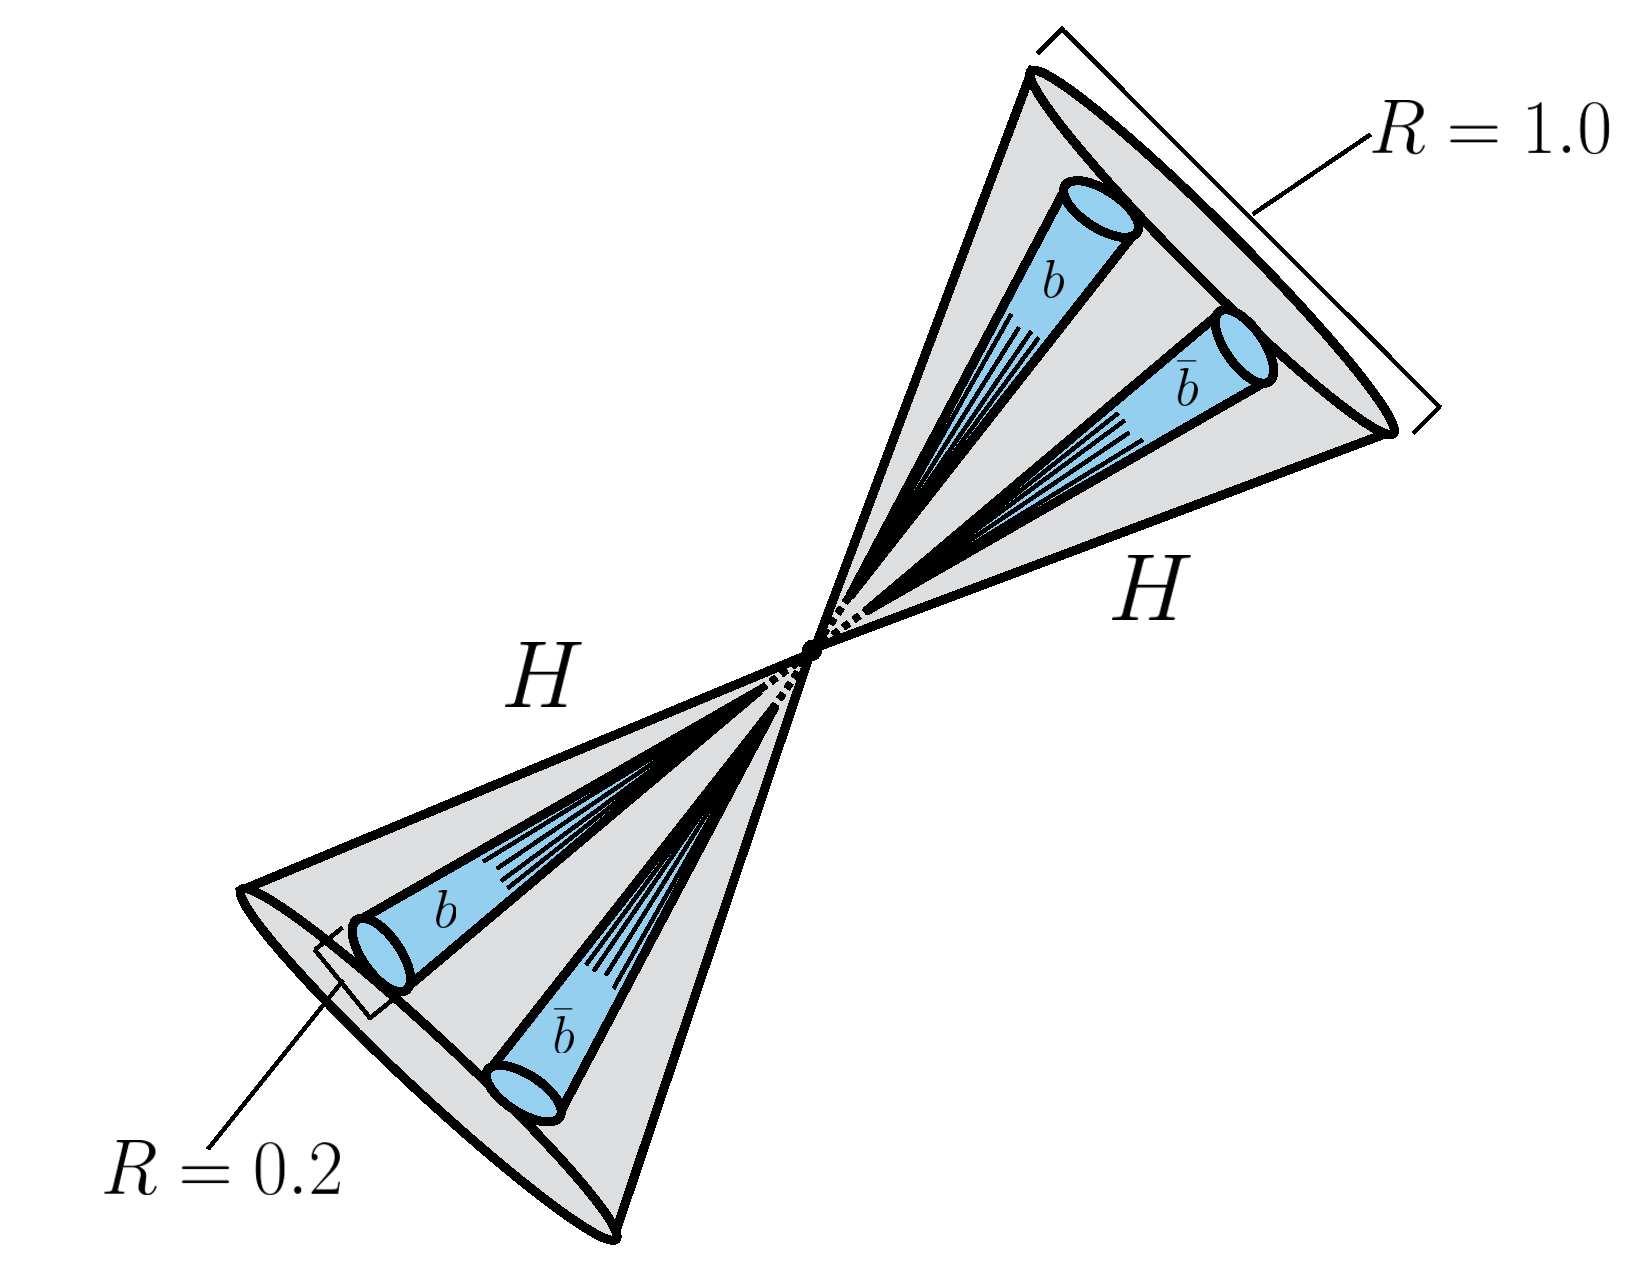
\includegraphics[width=\textwidth]{figures/Boosted_HH_cartoon}
  \caption{Illustration of the boosted selection requirements on Higgs candidates. Each large-radius calorimeter jet (Higgs candidate) must contain two track jets}
  \label{fig:BoostedCartoon}
\end{figure}

The first requirement in the boosted selection is for $\geq 2$ large radius jets satisfying the selections outlined above. The two highest momentum large-R jets in the event are referred to as ``Higgs candidates". The leading jet is required to have $\pT > 350 \GeV$. 

Track jets satisfying the object selections are matched to Higgs candidate jets via ghost association~\cite{GhostAssociation}. Each Higgs candidate must have at least $2$ track jets associated with it. These basic requirements are illustrated in figure~\ref{fig:BoostedCartoon}

The QCD multijet background produces less central jets than high mass resonances, so there is an additional requirement that the two Higgs candidates be close together in $\eta$. The large-R jets are required to satisfy $|\Delta\eta(JJ)| < 1.7$. 

The final set of requirements ensures that the Higgs candidates are consistent with expected properties of the $125.0 \GeV$ Higgs. First, a variable ($\Xhh$) is defined to measure the consistency of both of the Higgs candidate jets with the SM Higgs mass. This is shown in equation~\ref{eqn:Xhh}. 

\begin{equation}
\label{eqn:Xhh}
\Xhh = \sqrt{\left(\frac{M_J^{\rm lead} - 124 \GeV}{0.1 M_J^{\rm lead}}\right)^2 + \left(\frac{M_J^{\rm sublead} - 115 \GeV}{0.1 M_J^{\rm sublead}}\right)^2}
\end{equation}

The mass values in the $\Xhh$ formula are optimized to maximize signal efficiency. The sub-leading jet typically has a lower mass due to semi-leptonic $b$ decays and final state radiation. $\Xhh$ effectively acts as a $\chi^2$ measurement of the consistency of the two Higgs candidate masses with the signal hypothesis. The denominators of each term ($0.1M$) give the uncertainty on the mass measurement for the large radius jets. Events are required to satisfy $\Xhh < 1.6$. 

The last requirement applied is on the number of $b$-tagged track jets. There are two signal regions defined. The first requires exactly four $b$-tagged track jets, two in each Higgs candidate (known as the $4b$ signal region). At high resonance masses, this requirement is inefficient, so an additional signal region requiring only three $b$-tagged track jets is also defined (known as the $3b$ signal region). While this has a larger background it is also more efficient for high resonance masses. For both signal regions, threshold on MV2 score is chosen such that the algorithm is $77\%$ efficiency in finding true $b$-jets. Different working points were tested and this was found to be optimal. Appendix~\ref{AppendixA} has more details on this optimization. 

Before making the requirement on $\Xhh$, the masses of the Higgs candidates are corrected for semi-leptonic $b$ decays using muons with the criteria outlined in the previous section. Any muons within a $\Delta R < 0.2$ of a $b$-tagged track jet have their four-momenta added to the four-momentum of the Higgs candidate. This correction does not affect the pre-selection requirements but does affect the $\Xhh$ requirement and the final invariant mass distribution used. 

\begin{figure}[h!]
  %\vspace{20pt}
  \centering
  \captionsetup{justification=centering}

   \begin{subfigure}[t]{0.5\textwidth}
        \centering
        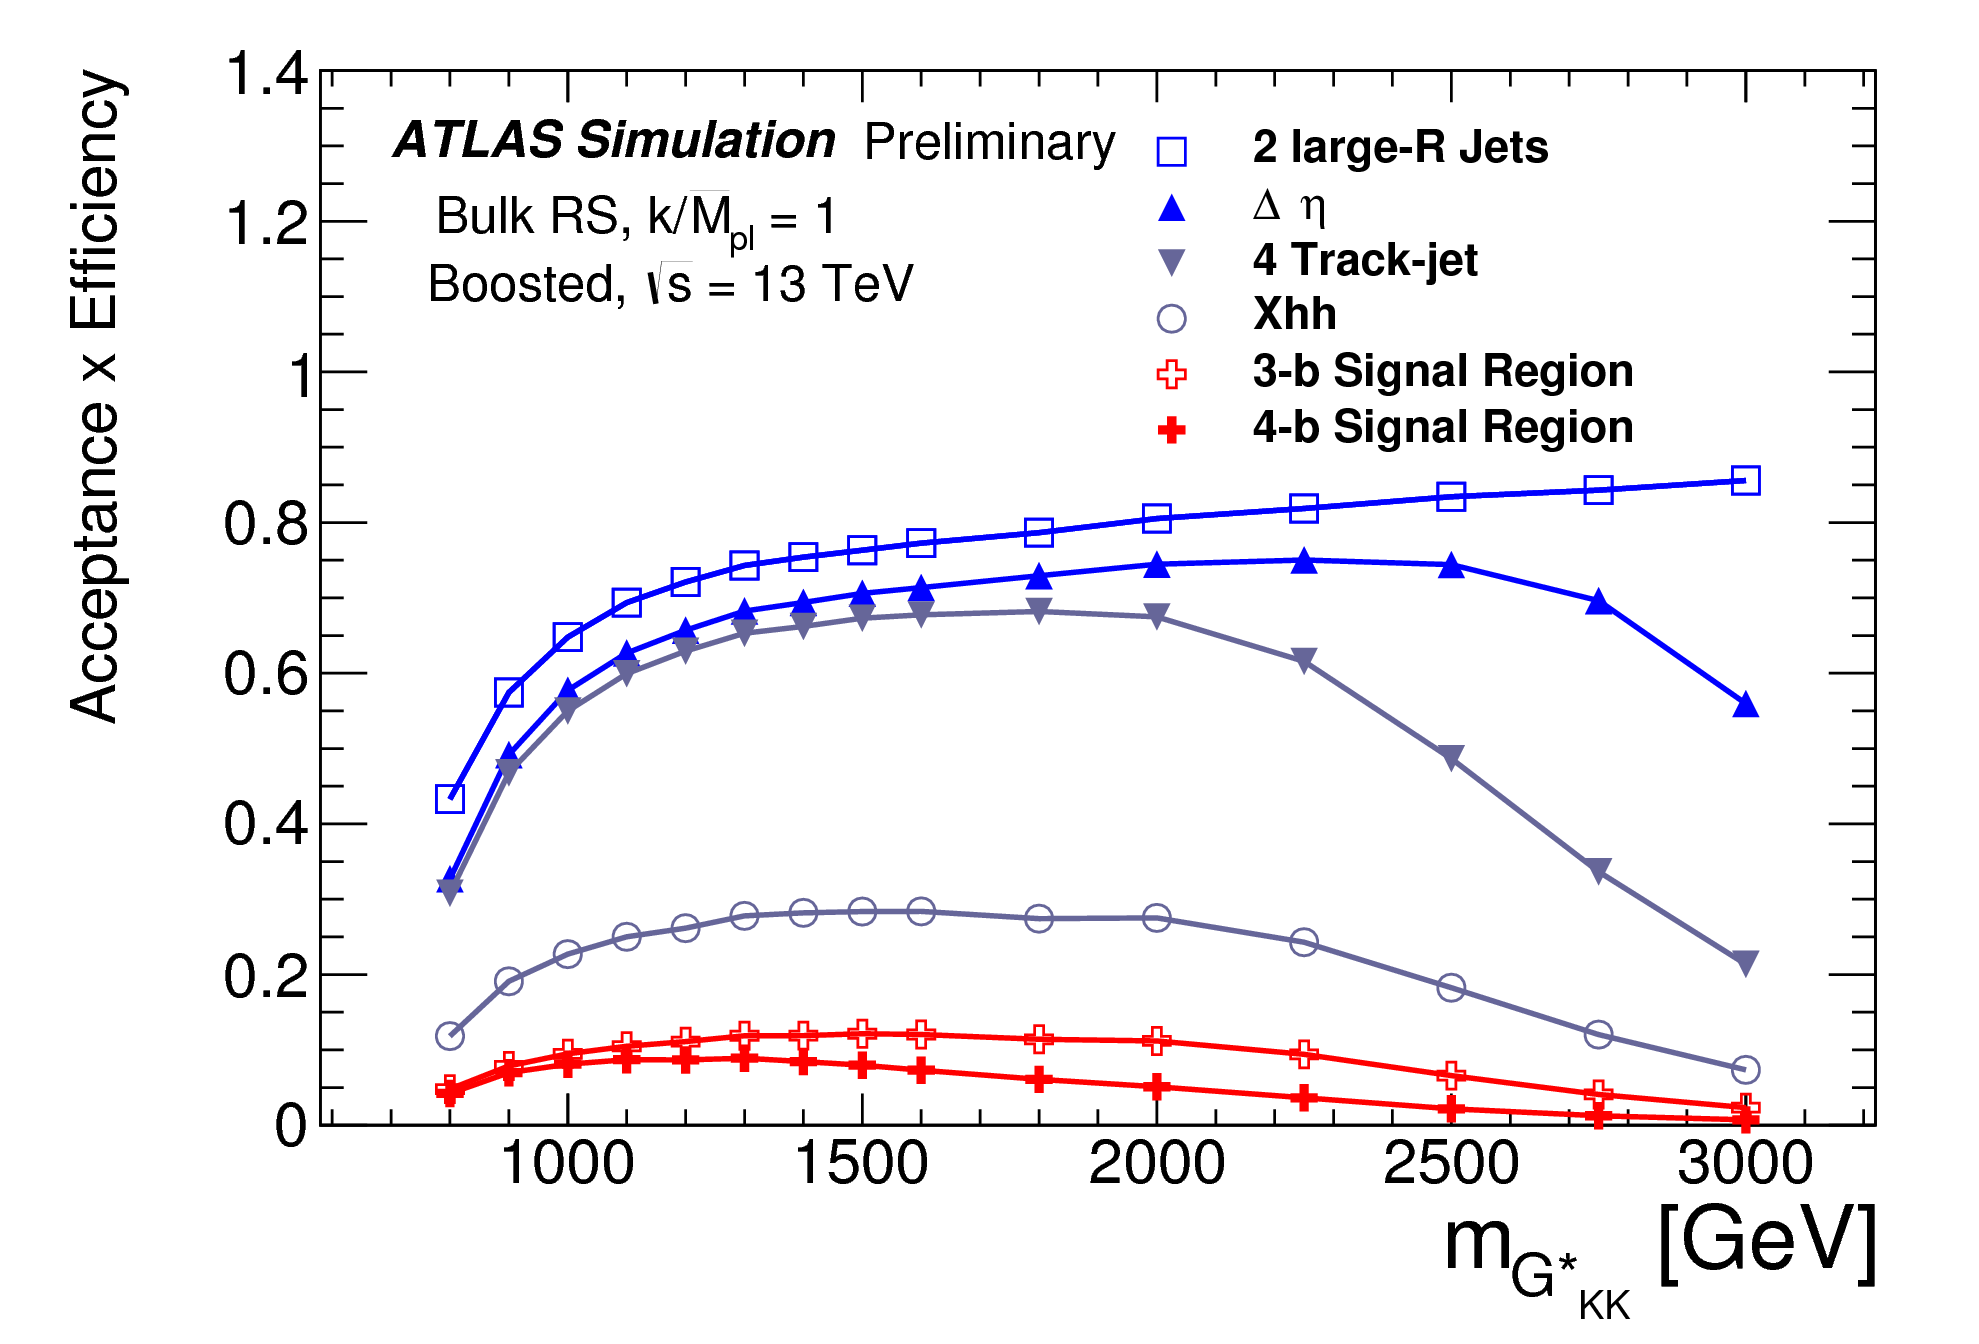
\includegraphics[width=\textwidth]{figures/4b_eff_RSG}
        \caption{}
    \end{subfigure}%
    \begin{subfigure}[t]{0.5\textwidth}
        \centering
        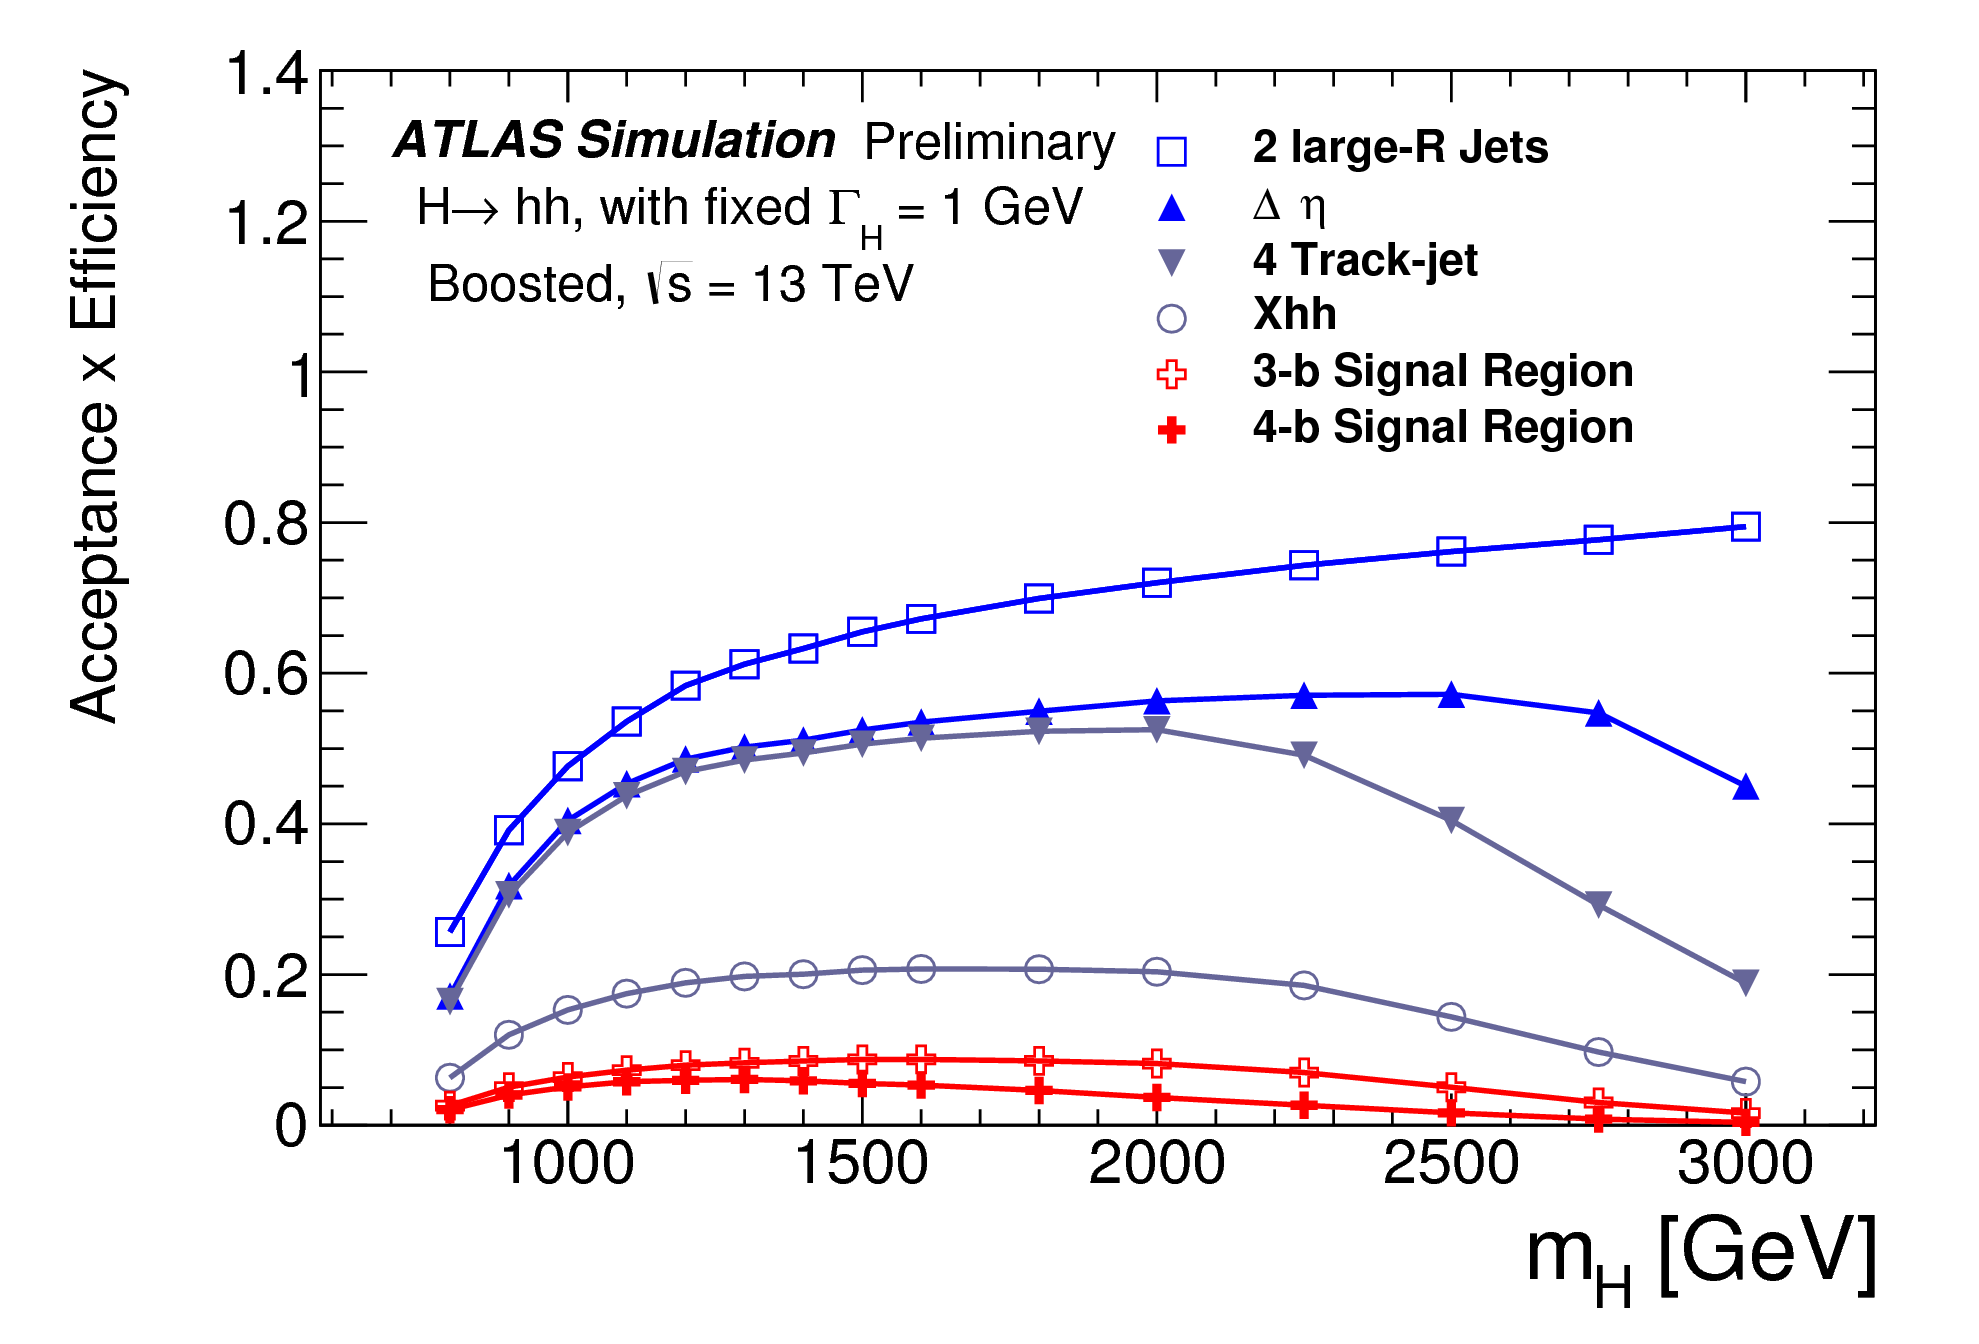
\includegraphics[width=\textwidth]{figures/4b_eff_H}
        \caption{}
    \end{subfigure}

   \caption{Acceptance $\times$ efficiency as a function of mass for (a) RSG and (b) narrow heavy scalar signal models~\cite{4bconf}.}
  \label{fig:4beff}
\end{figure}

Figure~\ref{fig:4beff} shows the product of acceptance and efficiency as a function of mass for both the RSG and narrow heavy scalar resonance signal models. After $m_{X} > 1 \TeV$, the efficiency of the $4b$ requirement begins to decline. After $m_{X} > 2 \TeV$, the efficiency of requiring two track jets in each Higgs candidate begins to decline as well. Both of these behaviors illustrate the difficulty of reoslving the merged decay products at high mass. More details on the degradation of the $b$-tagging efficiency at high masses are shown in appendix~\ref{AppendixB}. 

Figure~\ref{fig:3bvs4b} shows a more detailed comparison of the signal efficiency in the $3b$ vs $4b$ signal regions for the RSG model. The efficiencies shown here are relative to all prior selection requirements. 

\begin{figure}[h!]
  %\vspace{20pt}
  \centering
  \captionsetup{justification=centering}

  %\hspace*{-32pt}
  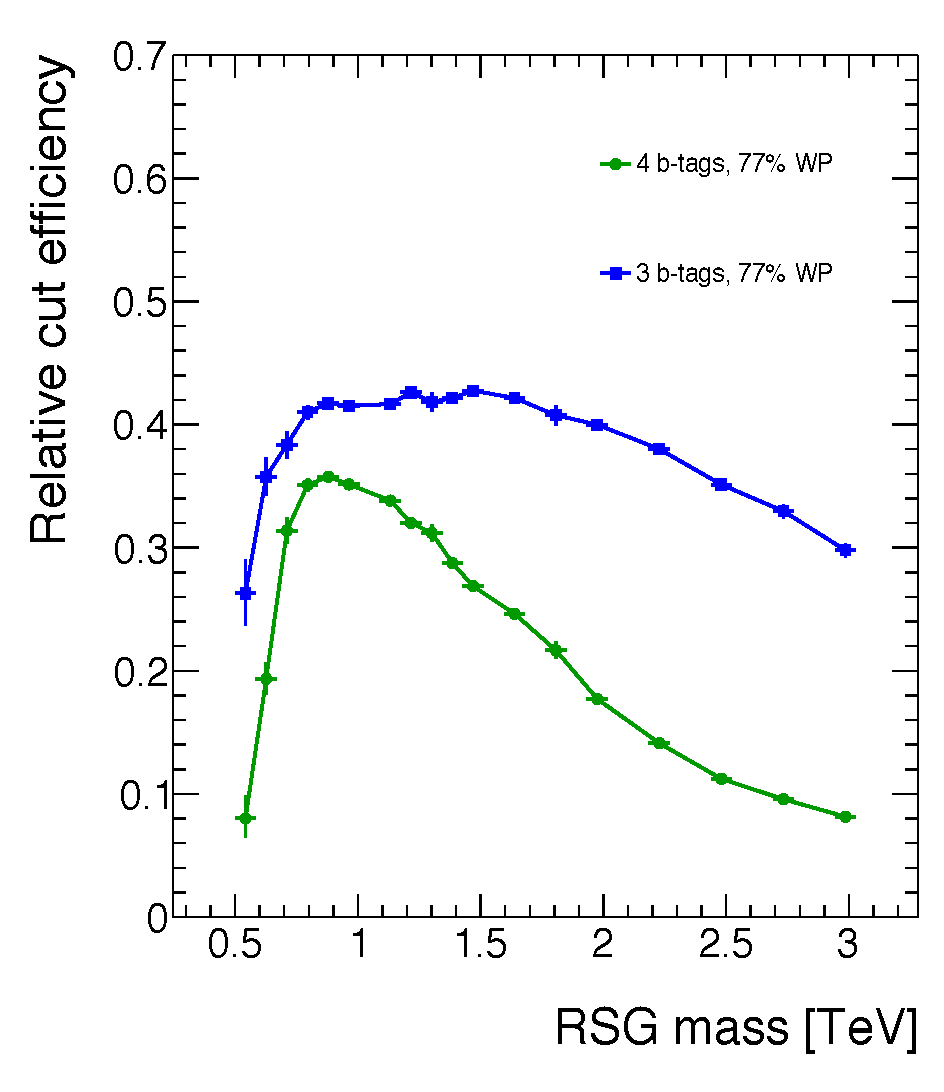
\includegraphics[width=0.5\textwidth]{figures/3bvs4b_eff}
  \caption{Efficiency of requiring $3$ or $4\,$ $b$-tagged track jets vs. RSG mass. The efficiency quoted is relative to the previous selection requirements (rather than an absolute efficiency). }
  \label{fig:3bvs4b}
\end{figure}

The final discriminating variable used in the boosted analysis is $M_{2J}$, the invariant mass of the two Higgs candidates. In order to improve the mass resolution, the four-momenta of each Higgs candidate are scaled by $m_{h}/M_{J}$. The effect of this correction is small in the boosted analysis but is done for consistency with the resolved selection. 

Table~\ref{tab:4bcutflow} shows the effect of the selection requirements on signal and background simulations as well as data. 

\begin{table}[h!]
\centering
\captionsetup{justification=centering}

%\begin{tabular*}{0.480\textwidth}{p{0.075\textwidth} p{0.180\textwidth} l}
\hspace{-10pt}
\begin{tabular}{c|c|c|c|c|c}
Selection & Data & \specialcell{$m_{\Gkk}$ \\ $=1$TeV} & \specialcell{$m_{\Gkk}$\\ $=2$TeV} & $t\bar{t}$ & $Z$+jets \\
\hline
N(fiducial large-R jets)$\geq 2$ & $2202396$ & $23.3$ & $0.48$ & $32345.2$ & $4255.7$ \\
leading large-R jet $p_{T}>350$ GeV & $1873741$ & $22.9$ & $0.48$ & $26511.7$ & $3649.9$ \\
Both large-R jet $m>50$ GeV & $1854625$ & $21.2$ & $0.47$ & $24369.8$ & $3575.8$ \\
Both large-R jet $p_{T}<1500$ GeV & $1853601$ & $21.2$ & $0.46$ & $24346.5$ & $3572.9$ \\
$|\Delta\eta(JJ)|<1.7$ & $1435273$ & $20.8$ & $0.44$ & $20751.0$ & $3265.8$ \\
$\geq 2$ track-jets per large-R jet & $1224727$ & $19.8$ & $0.40$ & $18234.5$ & $2692.6$ \\
\hline
3 $b$-tags, $X_{hh}<1.6$ & $316$ & $3.4$ & $0.067$ & $46.7$ & $2.0$ \\
\hline
4 $b$-tags, $X_{hh}<1.6$ & $20$ & $2.9$ & $0.030$ & $1.4$ & $0.0$ \\
\hline
\end{tabular}

\caption{
Effect of boosted selection on data, RSG signal models, $\ttbar$, and $Z$+jets. The numbers from simulation are normalized with the MC generator cross section and do not take into account the data driven estimates described in section~\ref{sec:dd4b}~\cite{Qi}.
}
\label{tab:4bcutflow}
\end{table}

\section{Data-driven background estimation}
\label{sec:dd4b}

The largest background to this final state is QCD multijet production, constituting $80$-$90$\% of the total background. Because of the difficulties in modeling higher order QCD processes, this background is estimated with a fully data-driven method. The only other non-negligible background is $\ttbar$, contituting the other $10$-$20$\%\footnote{The $Z$+jets background is a sub-percent level contribution}.  Due to the presence of $\ttbar$ in the sideband region where the QCD background will be estimated, the normalization of the QCD and $\ttbar$ backgrounds are simultaneously estimated. 

\subsection{Mass region definitions}

The first step in the data-driven background estimate is to define a sideband mass region where the background normalization can be derived. Additionally, a control region is defined where the background estimate can be validated. The control (CR) and sideband (SB) regions are defined using a radial distance in the two-dimensional large-R jet mass plane, $\Rhh$, which is defined in equation~\ref{eqn:Rhh}.

\begin{equation}
\label{eqn:Rhh}
\Rhh = \sqrt{\left(M_{J}^{\rm lead} - 124 \GeV\right)^2 + \left(M_{J}^{\rm sublead} - 115 \GeV\right)^2}
\end{equation}

Events in the sideband region are required to fail the signal region $\Xhh < 1.6$ requirement and have $\Rhh > 35.8 \GeV$. The control region consists of those events which are not in the signal or sideband regions. Figure~\ref{fig:MassRegions} shows the definition of the signal, control, and sideband mass regions.

\begin{figure}[h!]
  %\vspace{20pt}
  \centering
  \captionsetup{justification=centering}

  %\hspace*{-32pt}
  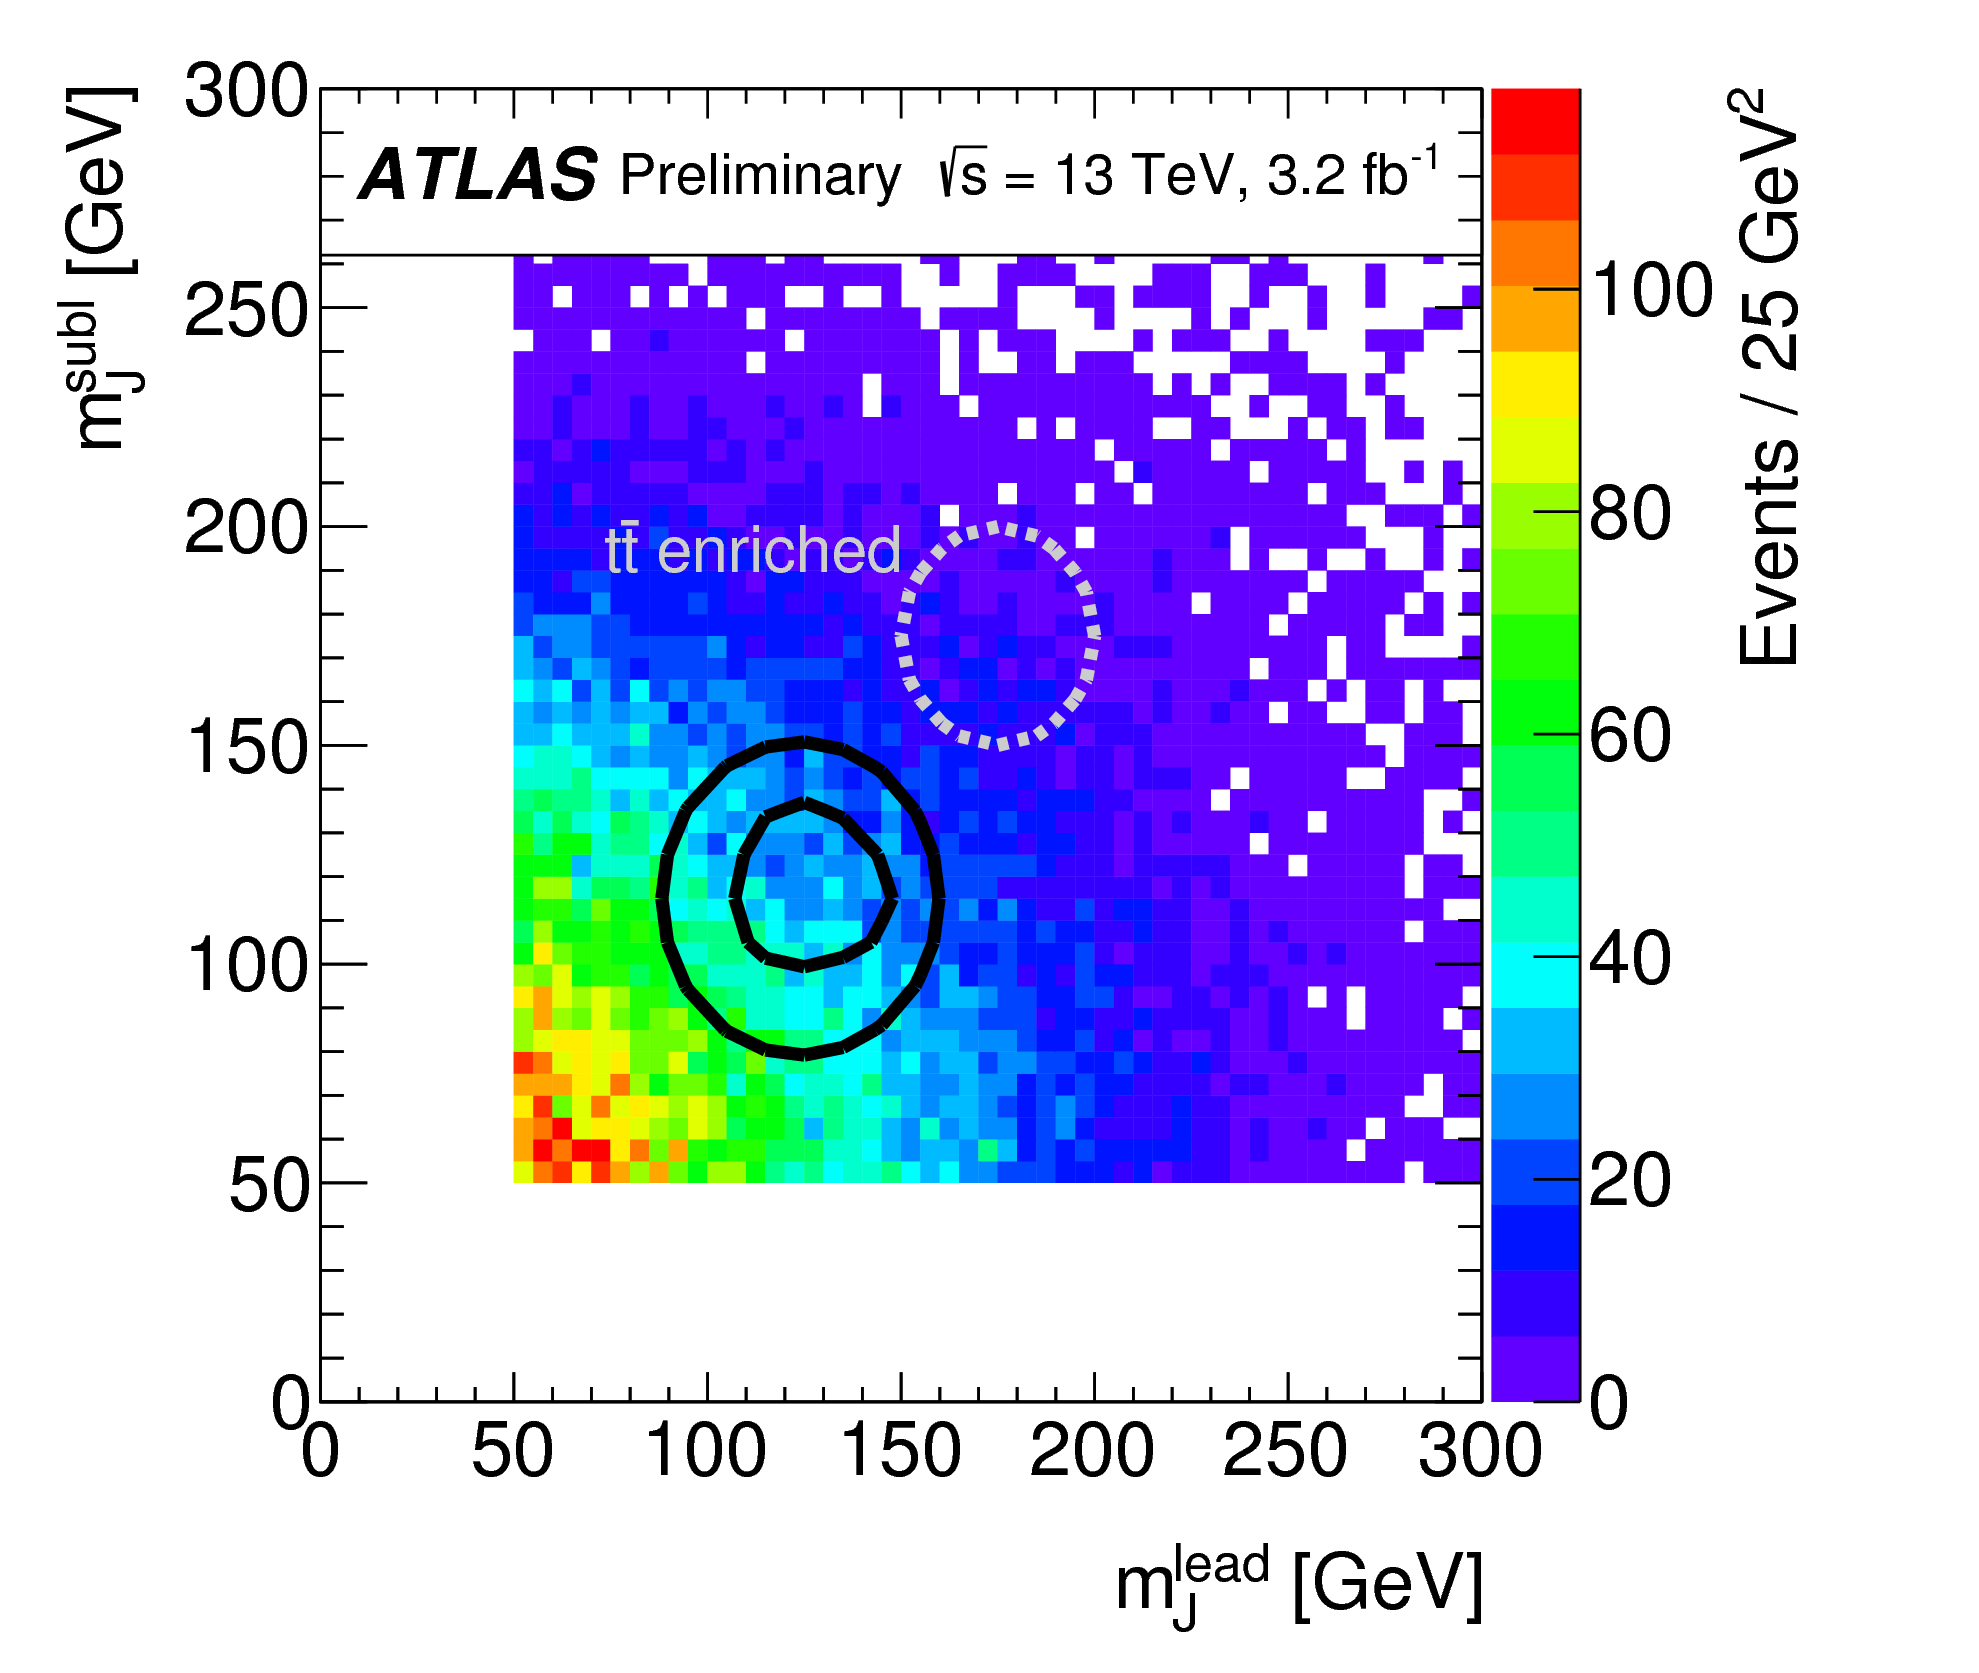
\includegraphics[width=0.6\textwidth]{figures/MassRegions}
  \caption{$M_{J}^{\rm sublead}$ vs. $M_{J}^{\rm lead}$ in a $2\,b$-tag data sample. The signal region is defined by the inner black contour ($\Xhh < 1.6$) and the sideband region is defined by the outer contour ($\Rhh > 35.8 \GeV$). The region between the black contours is the control region. The mass region which is enriched in $\ttbar$ background is also shown for illustration.~\cite{4bconf}}
  \label{fig:MassRegions}
\end{figure}

Table~\ref{tab:MassRegions} summarizes the mass region selections for the three different regions used in the analysis.

\begin{table}[h!]
\centering
\captionsetup{justification=centering}

%\begin{tabular*}{0.480\textwidth}{p{0.075\textwidth} p{0.180\textwidth} l}
\hspace{-10pt}
\begin{tabular}{|c|c|c|}
\hline
Region & Requirement & Notes \\
\hline
Signal Region (SR) & $\Xhh < 1.6$ & - \\ \hline
Control Region (CR) & $\Rhh < 35.8\GeV$ and $\Xhh > 1.6$ & \specialcell{Used for validation\\of background estimates} \\ \hline
Sideband Region (SB) & $\Rhh > 35.8 \GeV$ & \specialcell{Used to derive\\background normalization} \\
\hline
\end{tabular}
\caption{
Mass region definitions used for background estimation
}
\label{tab:MassRegions}
\end{table}

\subsection{Background estimation}

The method for estimating the background in this analysis is similar to the ABCD method presented in Chapter 5. In this case, the two handles used to define different regions for the estimate are the number of $b$-tagged track jets and the mass regions. A region requiring exactly two $b$-tagged track jets in one large-R jet (referred to as the $2$-tag or $2b$ region) is defined for use in the background estimate. The number of expected background events in the $3b$ and $4b$ signal regions is then given by equation~\ref{eqn:4b_bkg}.

\begin{equation}
\label{eqn:4b_bkg}
N_{\rm bkg}^{\rm 3(4)-tag, SR} = \muM N_{\rm Multijet}^{\rm 2-tag, SR} + \beta_{\ttbar} N_{\ttbar}^{\rm 3(4)-tag, SR} + N_{Z+ \rm jets}^{\rm 3(4)-tag, SR}
\end{equation}

In this equation, $N_{\rm bkg}^{\rm 3(4)-tag}$ is the expected number of background events in the $3b$ or $4b$ signal regions. $N_{\rm Multijet}^{\rm 2-tag}$ is the number of multijet events in the $2$-tag region. $N_{\ttbar}^{\rm 3(4)-tag}$ is the number of $\ttbar$ events predicted in the MC for the $3b$ or $4b$ signal region, and the variable is similarly defined for the $Z$+jets background. The $\beta_{\ttbar}$ parameter is a scale factor used to correct the normalization of the $\ttbar$ estimate in the signal region. $\muM$ is an extrapolation factor that is derived in the sideband region and used to estimate the ratio of $2$-tag events to $3$($4$)-tag events in the signal region. It is defined in equation~\ref{eqn:4bmu}.

\begin{equation}
\label{eqn:4bmu}
\muM = \frac{N_{\rm Multijet}^{\rm 3(4)-tag, SB}}{N_{\rm Multijet}^{\rm 2-tag, SB}} = \frac{N_{\rm data}^{\rm 3(4)-tag, SB} - \beta_{\ttbar} N_{\ttbar}^{\rm 3(4)-tag, SB} - N_{Z+ \rm jets}^{\rm 3(4)-tag, SB}}{N_{\rm data}^{\rm 2-tag, SB} - \beta_{\ttbar} N_{\ttbar}^{\rm 2-tag, SB} - N_{Z+ \rm jets}^{\rm 2-tag, SB}}
\end{equation}

The $\ttbar$ scale factor ($\beta_{\ttbar}$) and the QCD multijet extrapolation factor ($\muM$) are estimated together in a simultaneous fit in the sideband region. Then, the number of events in the $2$-tag signal region is used, along with the $\ttbar$ estimate in the $3b$ and $4b$ signal regions and $\muM$, to estimate the total number of background events in the two final signal regions. The shape of the final discriminant $M_{2J}$ is also taken from the $2$-tag signal region where there are more statistics. This method is illustrated graphically in figure~\ref{fig:4b_bkg_cartoon}.

\begin{figure}[h!]
  %\vspace{20pt}
  \centering
  \captionsetup{justification=centering}

  %\hspace*{-32pt}
  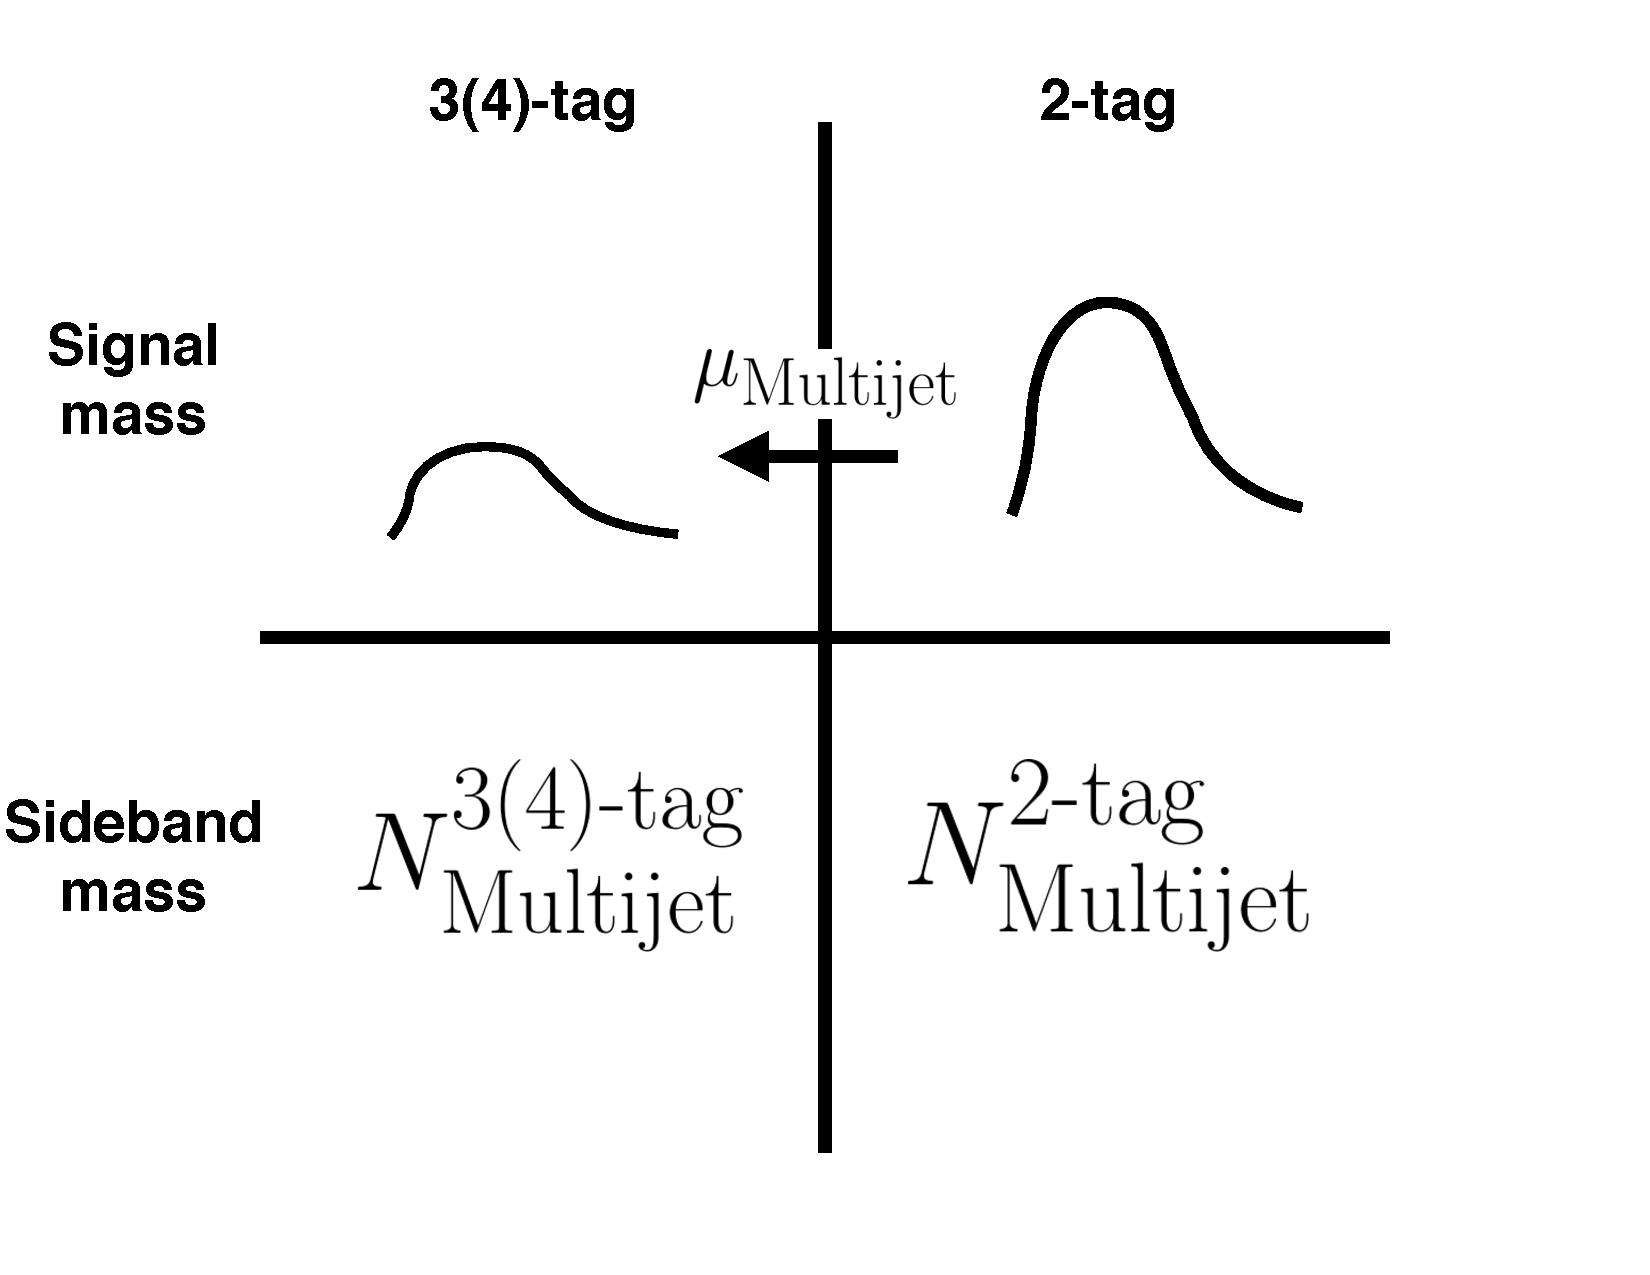
\includegraphics[width=0.6\textwidth]{figures/4b_bkg_cartoon}
  \caption{An illustration of the data-driven background estimation technique for the boosted analysis}
  \label{fig:4b_bkg_cartoon}
\end{figure}

In the $3b$ region, the fit yields values of $\muM = 0.160 \pm 0.03$ and $\beta_{\ttbar} = 1.02 \pm 0.09$. In the $4b$ region, the fit gives $\muM = 0.0091 \pm 0.0007$ and $\beta_{\ttbar} = 0.82 \pm 0.39$. The uncertainties quoted are statistical only. The larger uncertainties in the $4b$ values indicate the lower statistics available in that region. 

Figure~\ref{fig:4b_sideband} shows the distributions of data and background estimates in the $3b$ and $4b$ sideband regions after the background fit has been done. The normalizations are constrained from the fit to match that of the data, but good modeling of the shape of the mass of the leading large-R jet is seen as well. The shapes of the kinematic distributions in the $4b$ region are taken from the $3b$ region due to the better MC statistics in that region. 

\begin{figure}[h!]
  %\vspace{20pt}
  \centering
  \captionsetup{justification=centering}

   \begin{subfigure}[t]{0.5\textwidth}
        \centering
        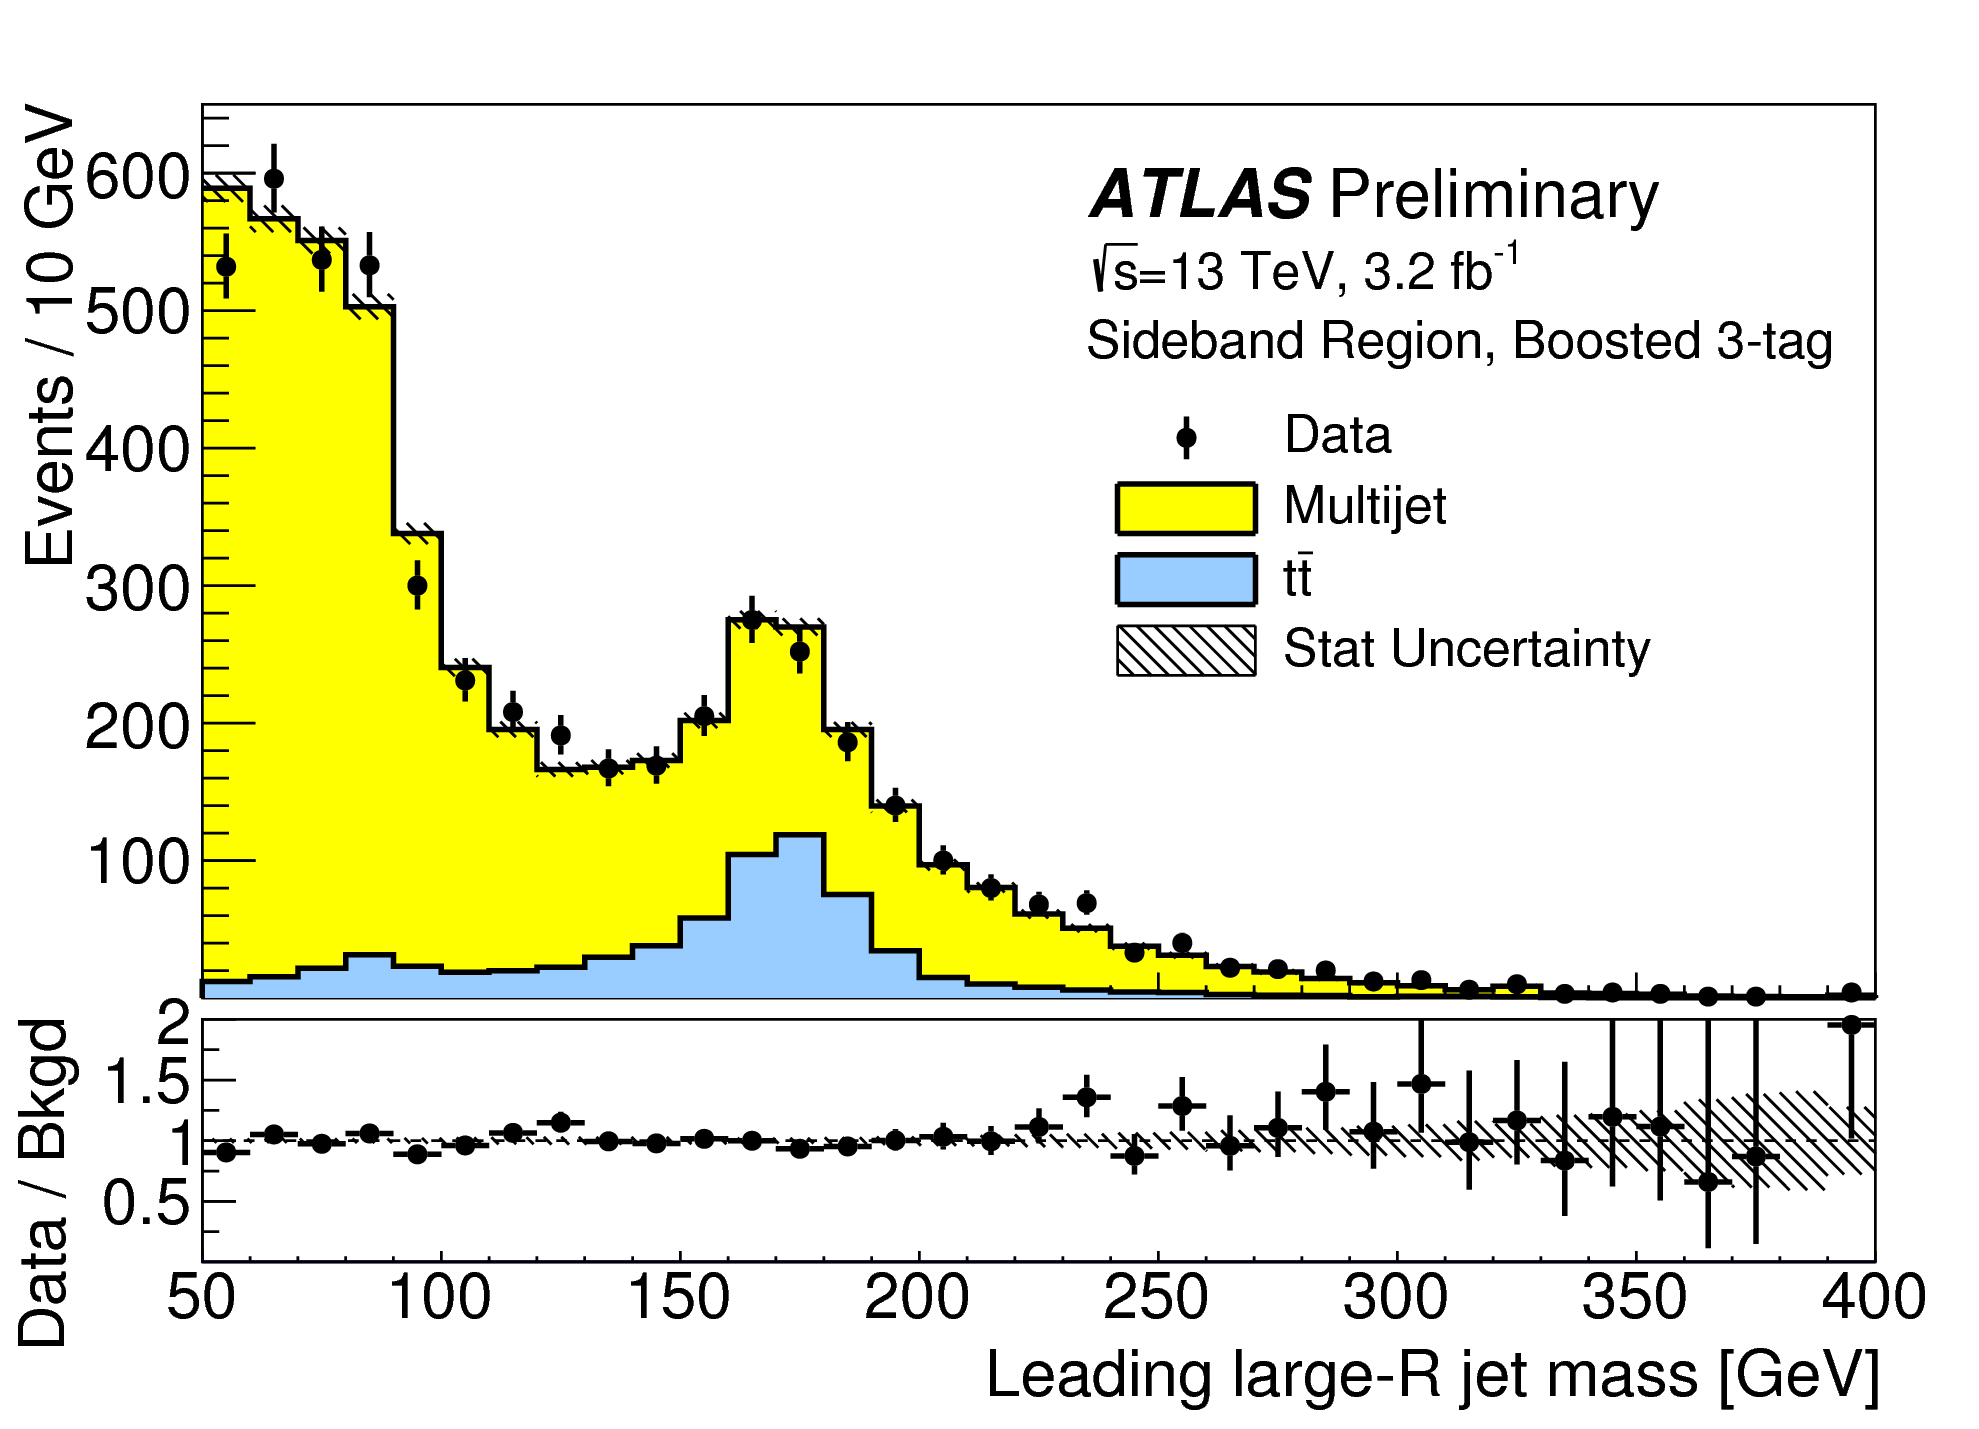
\includegraphics[width=\textwidth]{figures/3b_sideband}
        \caption{}
    \end{subfigure}%
    \begin{subfigure}[t]{0.5\textwidth}
        \centering
        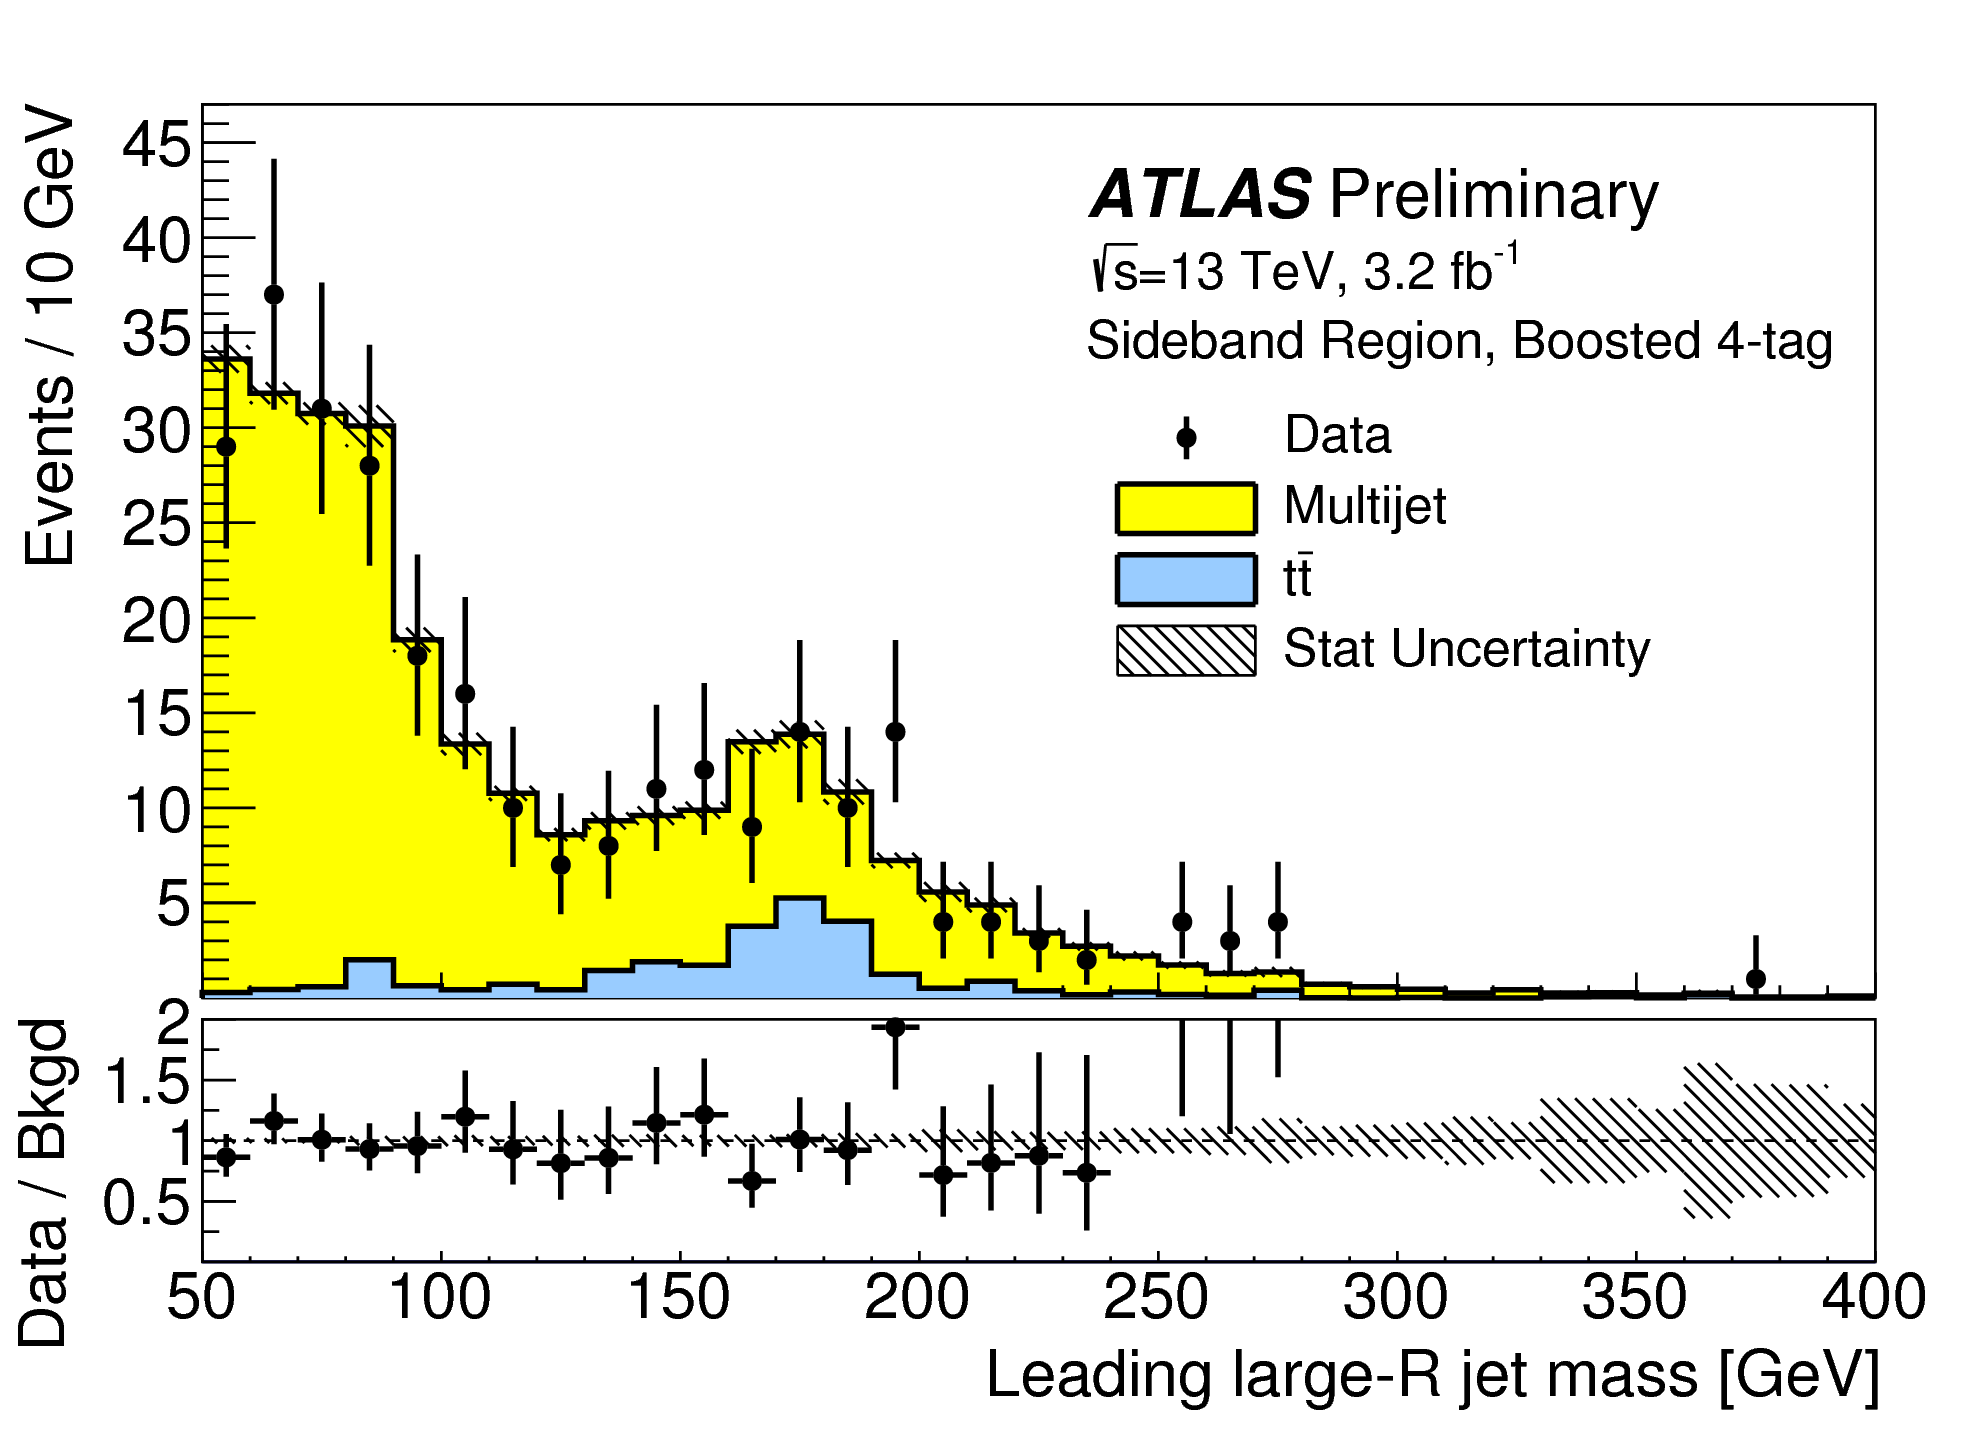
\includegraphics[width=\textwidth]{figures/4b_sideband}
        \caption{}
    \end{subfigure}

   \caption{Leading large-R jet mass in the $3b$ (a) and $4b$ (b) sideband regions. The multijet and $\ttbar$ backgrounds are estimated using the data-driven methods described above. Because their normalizations are derived in the sideband region, the total background normalization is constrained by default to match the normalization of the data~\cite{4bconf}.}
  \label{fig:4b_sideband}
\end{figure}

\subsection{Background shape fit}

As mentioned in the previous section, the background shape in the $3$-tag and $4$-tag signal regions is taken from the $2$-tag signal mass region. Due to the limited statistics available, the background shapes are additionally smoothed after being extrapolated to the $3$-tag and $4$-tag signal regions. Only the data in the range $900 < M_{2J} < 2000 \GeV$ is included in the fit due to the limited statistics available above $2 \TeV$. Both the $\ttbar$ and QCD multijet background are independently fit with an exponential shape, $y = e^{ax+b}$. Other shapes are considered and used for the systematic uncertainties. Table~\ref{tab:shape_fit} shows the fit values for the parameters. Because both the $3b$ and $4b$ QCD shapes come from the $2$-tag region, the slopes derived are very similar. 

\begin{table}[h!]
\centering
\captionsetup{justification=centering}

%\begin{tabular*}{0.480\textwidth}{p{0.075\textwidth} p{0.180\textwidth} l}
\hspace{-10pt}
\begin{tabular}{|c|c|c|}
\hline
 & $a$ & $b$ \\ \hline
QCD ($4b$) & $0.00545 \pm 0.00021$ & $5.44 \pm 0.24$ \\ 
$\ttbar$\,($4b$) & $0.00746 \pm 0.00021$ & $4.88 \pm 0.36$ \\ \hline
QCD ($3b$) & $0.00545 \pm 0.00021$ & $8.30 \pm 0.24$ \\ 
$\ttbar$\,($3b$) & $0.00746 \pm 0.00021$ & $8.58 \pm 0.36$ \\ \hline
\end{tabular}
\caption{
Parameters derived for exponential fit to background $M_{2J}$ shape in the $3b$ and $4b$ signal regions~\cite{Qi}
}
\label{tab:shape_fit}
\end{table}

\subsection{Validation of background estimate}

The background estimate can be validated by using the method to estimate the number of events in the control mass region rather than the signal mass region. Figure~\ref{fig:4b_control} shows the $M_{2J}$ distribution in the $3b$ and $4b$ control regions, comparing data and background estimates. In both cases, both the background shape and normalization are consistent with the data, indicating good agreement. The ratio of data to the background estimates is also fit to a line in the figure to test for any shape difference. The slope of the line is within $1\sigma$ (from the fit uncertainties) of flat, further indicating that the data is consistent with the background estimate in the control region. 

\begin{figure}[h!]
  %\vspace{20pt}
  \centering
  \captionsetup{justification=centering}

   \begin{subfigure}[t]{0.5\textwidth}
        \centering
        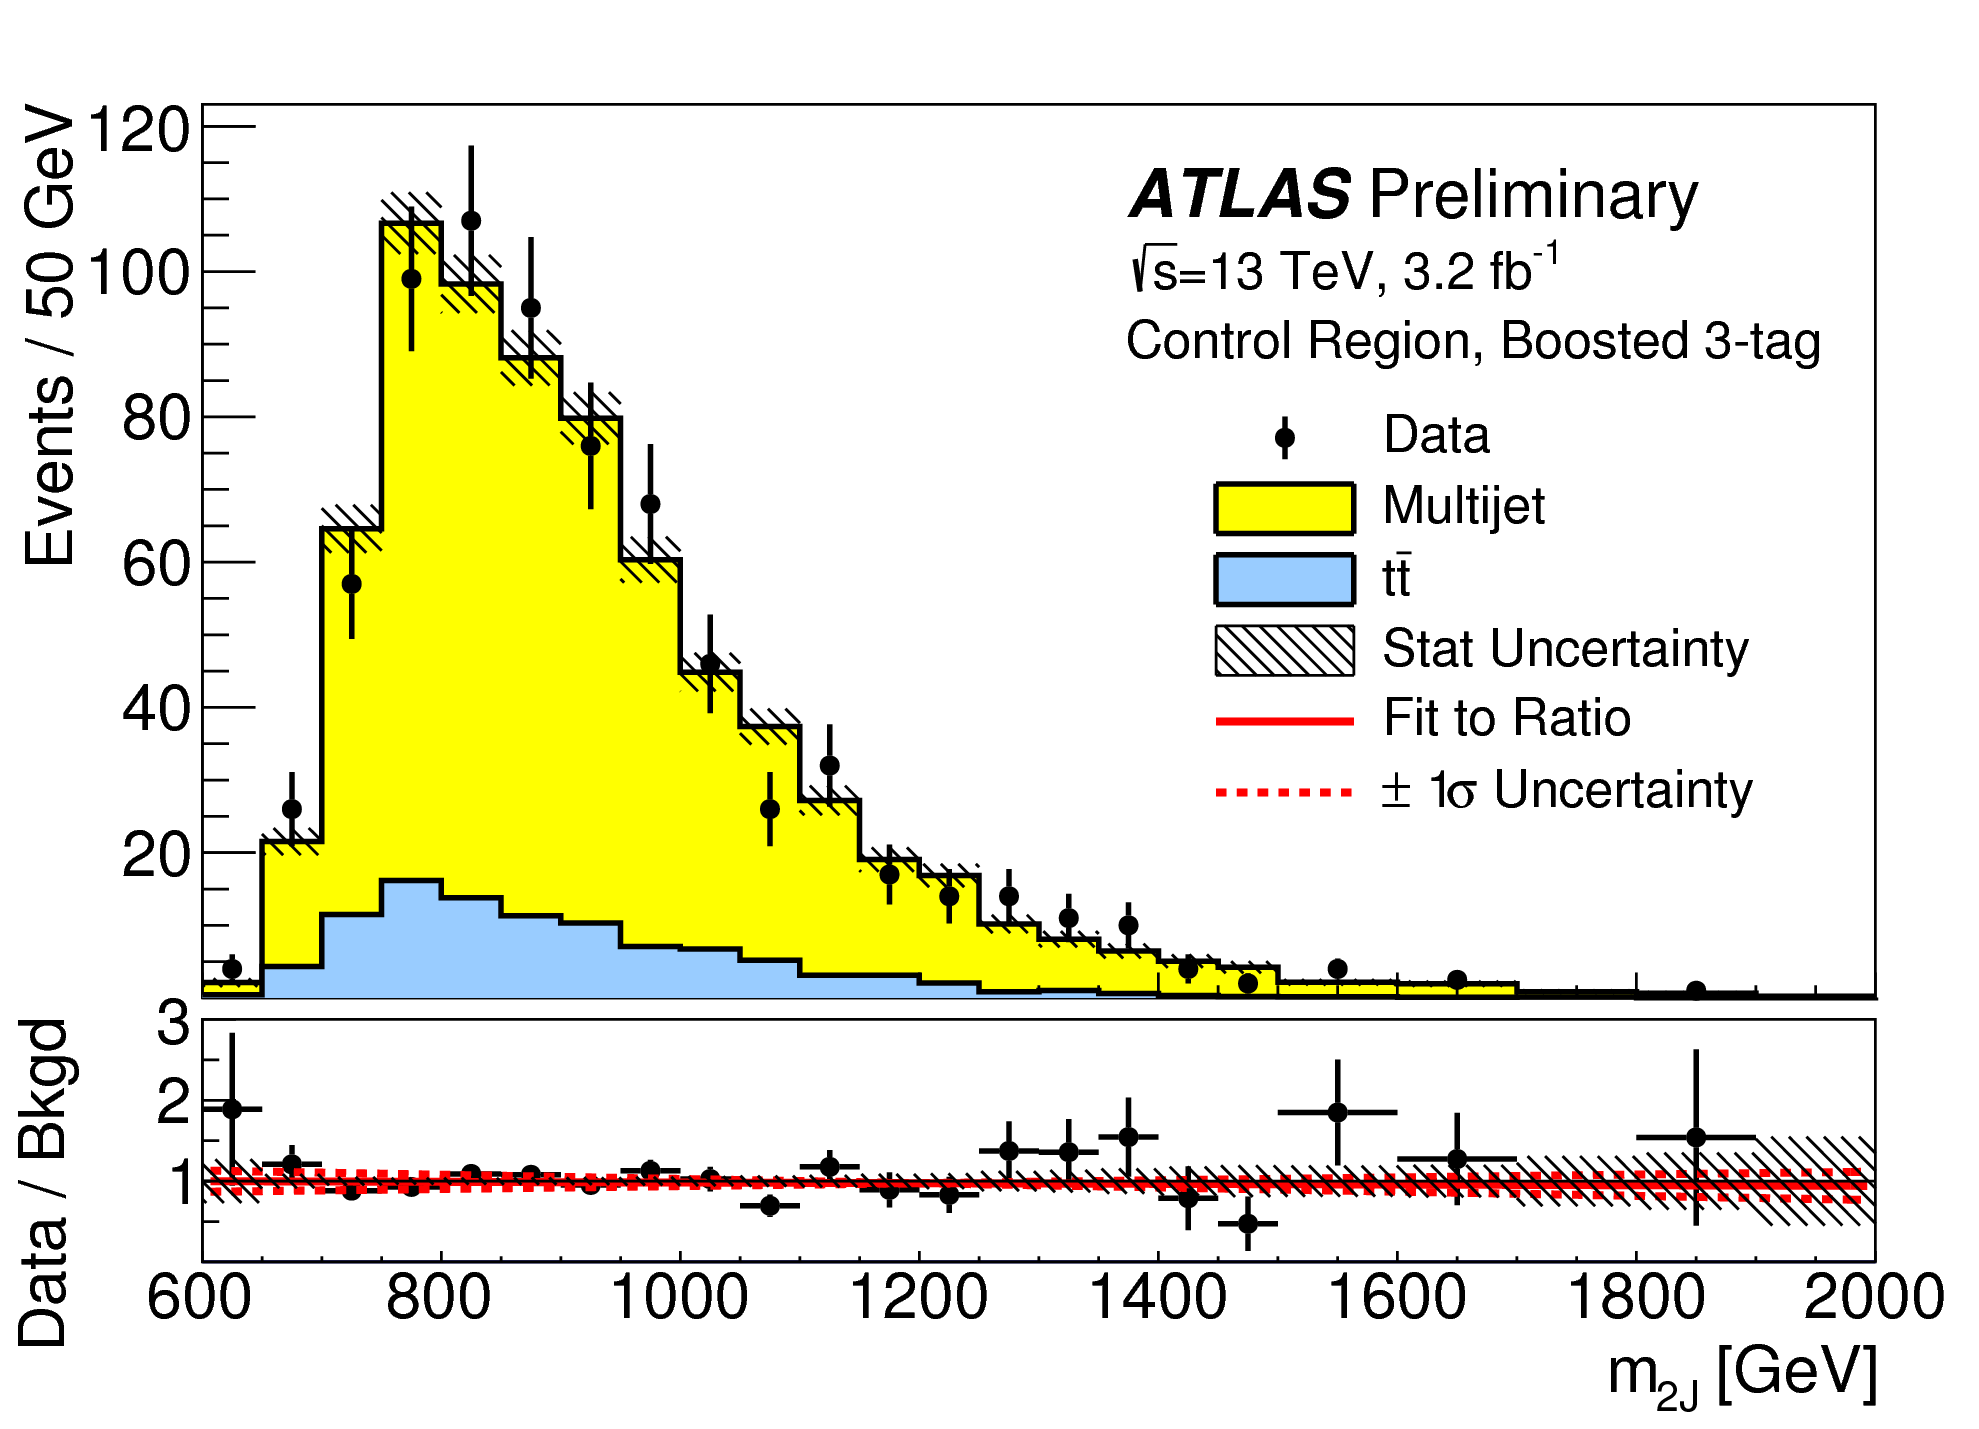
\includegraphics[width=\textwidth]{figures/3b_control}
        \caption{}
    \end{subfigure}%
    \begin{subfigure}[t]{0.5\textwidth}
        \centering
        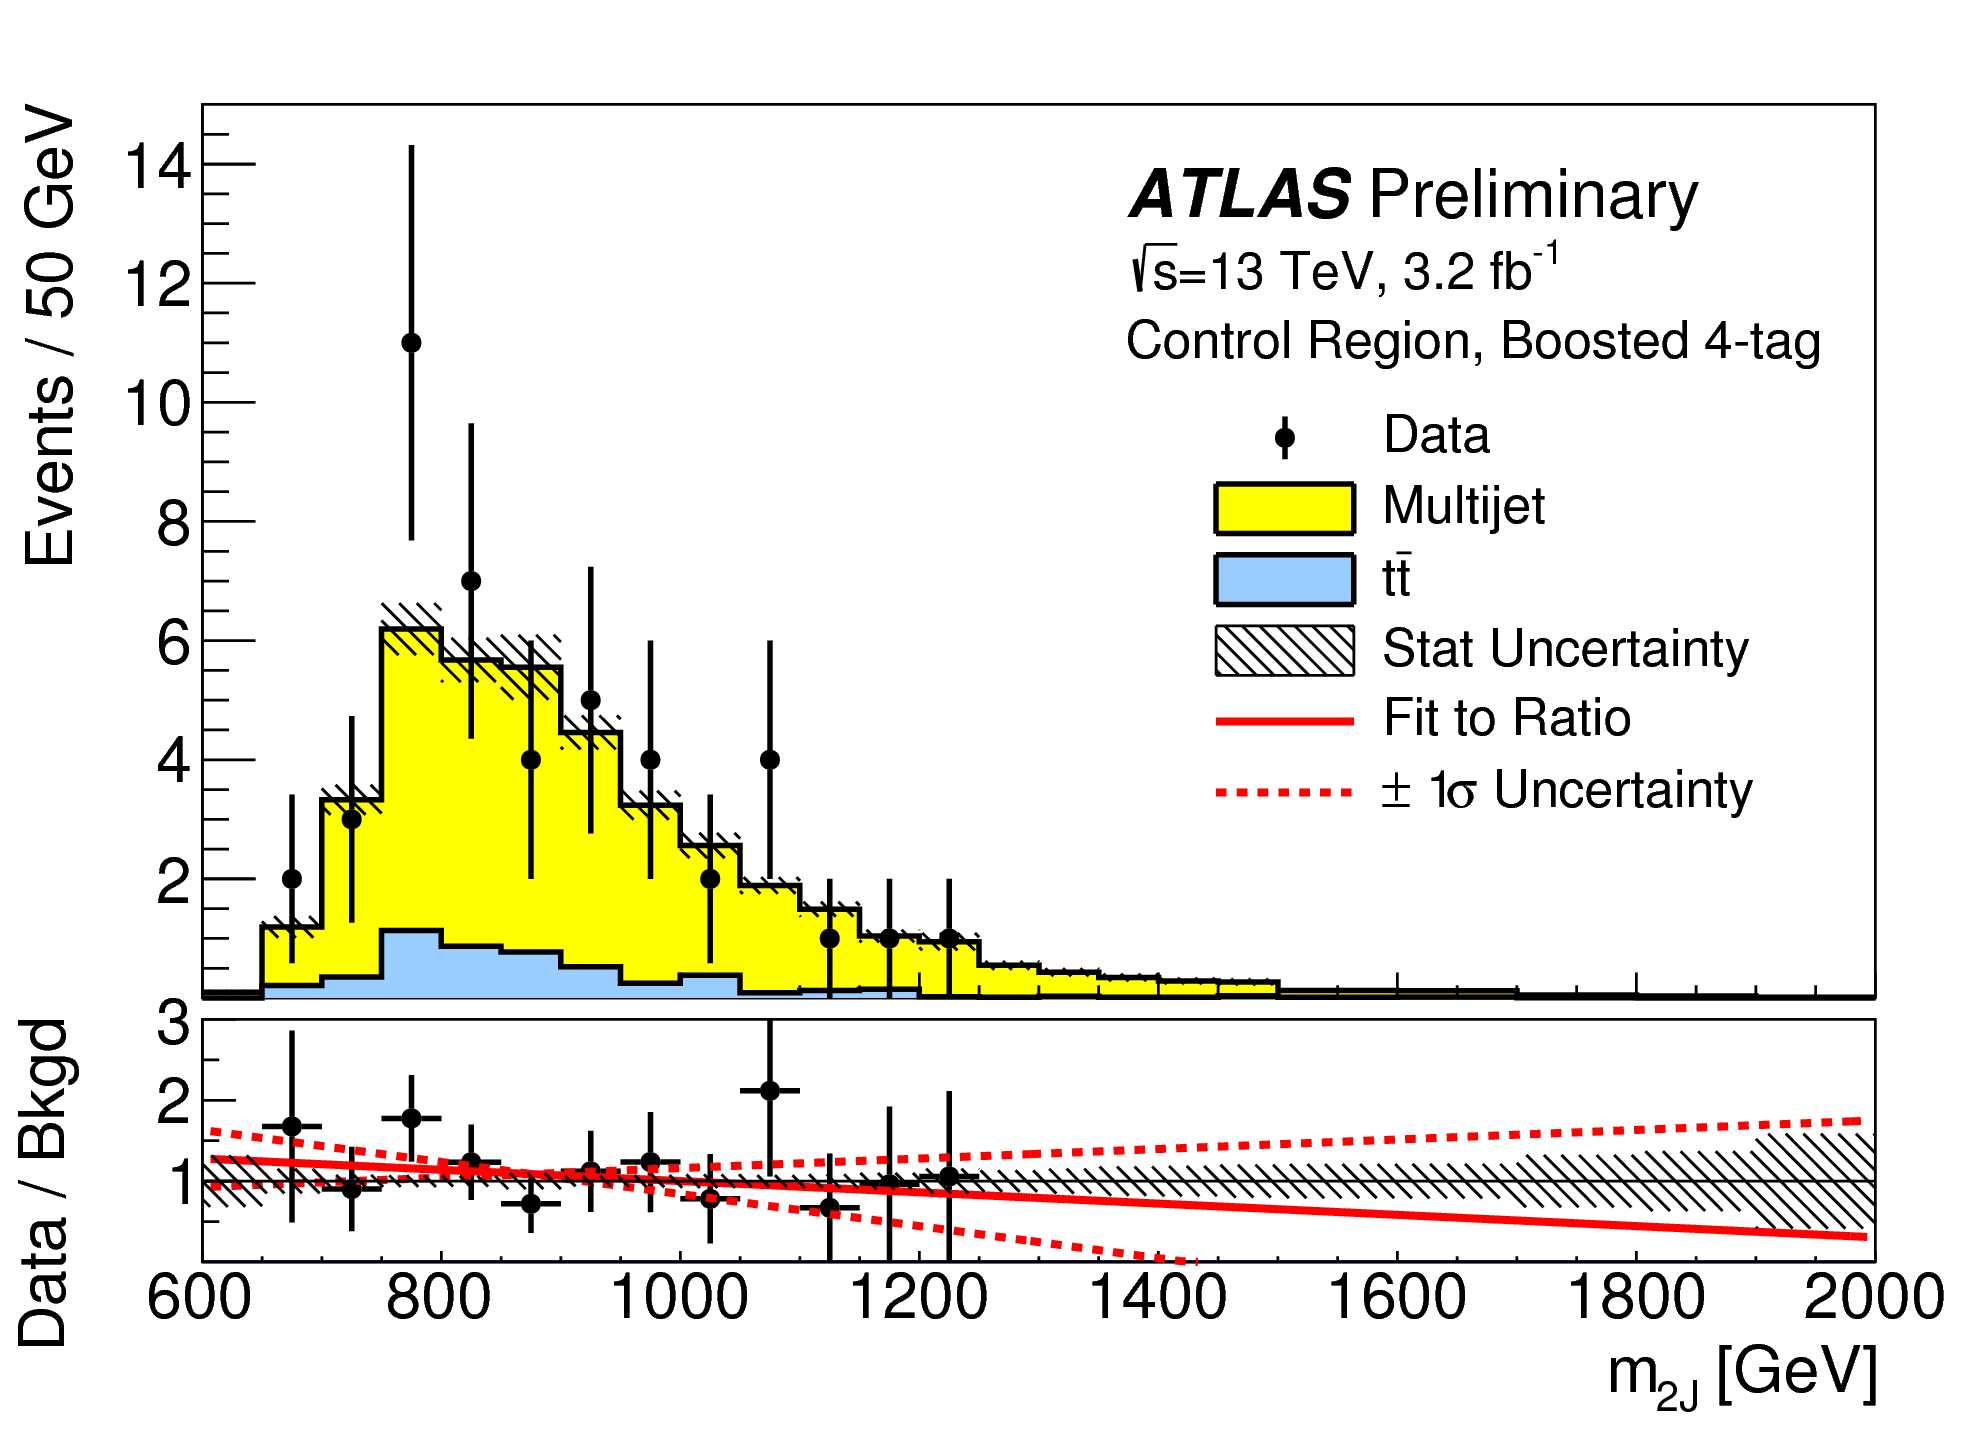
\includegraphics[width=\textwidth]{figures/4b_control}
        \caption{}
    \end{subfigure}

   \caption{Di-jet invariant mass ($M_{2J}$) in the $3b$ (a) and $4b$ (b) control regions. The multijet and $\ttbar$ backgrounds are estimated using the data-driven methods described above~\cite{4bconf}.}
  \label{fig:4b_control}
\end{figure}

Table~\ref{tab:4b_control} shows the yields in data and background estimates in the $3$-tag and $4$-tag sideband and control regions. Again, here, it can be seen that the total number of predicted background events from the data driven method is consistent with the number of data events in the region. 

\begin{table}[!ht]
\begin{center}
\begin{tabular}{ l c  c  }
\toprule
 Sample (3-tag) & Sideband Region       & Control Region  \\ 
\midrule
%Multijet        & 4327.9 $\pm$ 26.9     & 607.3  $\pm$  10.1  \\
Multijet        & $4328   \pm 27$       & $607  \pm  10$  \\
$\ttbar$          & $683.5  \pm 8.1$      & $99.6 \pm  3.1$ \\
$Z$+jets        & $31.8   \pm 3.7$      & $7.7  \pm  1.8$ \\
\midrule
%Total           & 5043.2 $\pm$ 28.3     & 714.6$\pm$  10.7 \\
Total           & $5043 \pm 28$     & $715\pm  11$ \\
\midrule
Data            & $5043$                  & $724$     \\  
\toprule
  Sample (4-tag) & Sideband Region      & Control Region  \\ 
\midrule
%Multijet         & 247.4 $\pm$ 1.5      & 34.71  $\pm$  0.58 \\
%\ttbar           & 28.4  $\pm$ 1.5      & 5.08   $\pm$  0.67 \\
%$Z$+jets         & 3.4   $\pm$ 1.2      & 0.55   $\pm$  0.45  \\
Multijet         & $247.4 \pm 1.5$      & $34.7  \pm  0.6$ \\
$\ttbar$           & $28.4  \pm 1.5$      & $5.1   \pm  0.7$ \\
$Z$+jets         & $3.4   \pm 1.2$      & $0.6   \pm  0.5$  \\
\midrule
Total            & $279.2 \pm 2.5$     & $40.3  \pm  1.0$  \\
\midrule
Data             & $279$                  & $45$     \\ 
\bottomrule
\end{tabular}
\caption{The number of events in data and predicted background events in the boosted $3$-tag and $4$-tag sideband and control
  regions. The uncertainties shown are statistical only.~\cite{4bconf}}
\label{tab:4b_control} 
\end{center}
\end{table}

\section{Systematic uncertainties}

The systematic uncertainties in this analysis can be divided into two broad categories. The first type is uncertainties associated with the modeling of the signal processes. The second type of uncertainty is associated with both the shape and normalization of the background prediction. 

\subsection{Signal modeling uncertainties}

The signal modeling uncertainty has three main components: theoretical uncertainty on the acceptance, experimental uncertainties on the large-R jets, and experimental uncertainties on the track jets related to $b$-tagging. In this analysis the experimental uncertainties are the most significant. 

The first uncertainty on signal modeling is the theoretical uncertainty on the acceptance. As explained in section~\ref{sec:theory_uncert_WW}, there are four components to this uncertainty. The first is related to missing higher order terms from the matrix element calculations which is estimated by varying the QCD renormalization and factorization scales. The second is uncertainty due to the PDF set used. The third is a generator uncertainty which is estimated by modifying the generator used to model the underlying event and hadronization. Finally, there is an uncertainty associated with the modeling of the initial state and final state radiation (ISR/FSR). The total theoretical uncertainty on the signal yield is $3\%$, and this is dominated by the ISR/FSR modeling.

There are uncertainties on the large-R jets in both the jet energy scale (JES) and jet energy resolution (JER) as well as the jet mass scale (JMS) and jet mass resolution (JMR). These are evaluated using $\sqrt{s} = 8 \TeV$ data from Run $1$ of ATLAS and extrapolated to the Run $2$ beam and detector conditions using MC\footnote{The uncertainties are correspondingly larger due to the uncertainty of this extrapolation.}. The details of these uncertainties can be found in reference~\cite{LargeRUncert}. 

Uncertainties on the track jets are related to the $b$-tagging efficiency. The total uncertainty on the signal yield due to $b$-tagging is evaluated by propagating variations of the $b$-tagging efficiency through the boosted selection requirements. The uncertainties are calculated jet-by-jet and paramaterized as a function of $b$-jet $\pT$ and $\eta$~\cite{BtagCalib1}. For high $\pT$ $b$-jets (with $\pT > 300 \GeV$), the uncertainties are extrapolated using MC simulation from the lower $\pT$ $b$-jets~\cite{BtagPaper}. 

Table~\ref{tab:BoostedSyst} shows the systematic uncertainties on the signal normalization for models with $m_{\Gkk} = 1.5 \TeV$ and both $c = 1$ and $c = 2$ as well as a narrow width heavy scalar. The dominant uncertainty comes from $b$-tagging and this uncertainty is larger in the $4$-tag region than the $3$-tag region. 

\begin{table}[ht!]
\begin{center} 
\begin{tabular}{  l  c  c  c  c }
\toprule
 Source          & Background    & \multicolumn{2}{c}{$\Gkk$} & $H$ \\
                 &         & $c = 1$ & $c = 2$  &     \\
\midrule
   Luminosity    &  -      &  $5.0$    &  $5.0$    & $5.0$ \\
\midrule
                \multicolumn{5}{c}{$3$-tag}  \\
\midrule
   JER           &  $<1$   &  $< 1$   &  $<1$   & $< 1$ \\
   JES           &  $2$    &  $<1$    &  $< 1$    & $<1$ \\
   JMR           &  $1$    &  $12$   &  $12$   & $11$  \\
   JMS           &  $5$    &  $14$   &  $13$   & $17$  \\
   $b$-tagging   &  $1$   &  $23$   &  $22$   & $23$  \\
   Theoretical   &  -      &  $3$    &  $3$    & $3$ \\
   Multijet Normalization      &  $3$    &  -      &  -      &  -  \\
   Statistical     &  $2$    &  $1$      &  $1$      &  $1$  \\
   \midrule
   Total         &  $7$    &  $31$   &  $30$   &  $33$ \\
   %% JER           &  0.4    &  0.6    &  0.4    & 1.0 \\
   %% JES           &  2.2    &  0.2    &  0.5    & 0.3 \\
   %% JMR           &  1.1    &  12.0   &  11.6   & 11.6  \\
   %% JMS           &  4.7    &  13.8   &  12.6   & 17.4  \\
   %% $b$-tagging   &  0.9    &  22.5   &  21.6   & 23.2  \\
   %% Theoretical   &  -      &  2.5    &  2.5    & 2.5 \\
   %% Multijet Normalization      &  3.1    &  -      &  -      &  -  \\
   %% Statistical    &  2.4    &  0.9      &  0.9      &  1.1  \\
   %% \midrule
   %% Total         &  6.7    &  31.0   &  29.7   &  33.1 \\
\bottomrule
                \multicolumn{5}{c}{$4$-tag}  \\
\midrule
   JER           &  $< 1$    &  $<1$  &  $<1$   & $<1$ \\
   JES           &  $< 1$    &  $<1$    &  $<1$    & $<1$ \\
   JMR           &  $4$    &   $12$   &  $13$   & $13$  \\
   JMS           &  $5$    &  $13$   &  $13$   & $14$  \\
   $b$-tagging   &  $2$    &  $36$   &  $36$   & $36$  \\
   Theoretical   &  -      &  $3$    &  $3$    & $3$ \\
   Multijet Normalization      &  $14$  &  -      &  -      &  -  \\
   Statistical    &  $3$    &  $1$      &  $1$      &  $1$  \\
   \midrule
   Total         &  $15$   &  $42$   &  $42$   & $43$ \\
   %% JER           &  0.5    &  <0.1   &  0.6    & 0.3 \\
   %% JES           &  0.6    &  0.3    &  0.5    & 0.2 \\
   %% JMR           &  3.8    &  11.5   &  13.0   & 12.8  \\
   %% JMS           &  4.7    &  12.9   &  12.5   & 14.0  \\
   %% $b$-tagging   &  1.6    &  36.3   &  36.0   & 36.4  \\
   %% Theoretical   &  -      &  2.5    &  2.5    & 2.5 \\
   %% Multijet Normalization      &  13.7   &  -      &  -      &  -  \\
   %% Statistical    &  2.5    &  1.1      &  1.2      &  1.4  \\
   %% \midrule
   %% Total         &  15.3   &  41.7   &  41.8   & 42.5 \\
\bottomrule
\end{tabular}
\caption{Summary of systematic uncertainties in the total background and signal event yields (expressed in $\%$) in the boosted $3$-tag and $4$-tag signal regions. Systematic uncertainties on the signal normalization are shown for models with $m_{\Gkk} = 1.5 \TeV$ and both $c = 1$ and $c = 2$ as well as a narrow width heavy scalar.
}
\label{tab:BoostedSyst}
\end{center}
\end{table}

\subsection{Background uncertainties}

Uncertainties on the QCD multijet background normalization and shape are estimated using the control mass region. As shown previously, the background predictions in the control region match with the data yields within the statistical uncertainty in both the $3$-tag and $4$-tag control regions. As an additional protection, the statistical uncertainty on the background prediction in the control region is assigned as a systmeatic uncertainty on the normalization of the QCD background. 

Additional robustness tests are done by varying the defintion of the control mass region and the $b$-tagging requirements used to define the $2$-tag sample. In all cases, the effect of the variations is found to be within the statistical uncertainties on the backgorund normalization in the control region. 

Shape uncertainties on the background are evaluated using two techniques. First, as shown in figure~\ref{fig:4b_control}, the ratio between the data and background prediction is fit with a linear function. The uncertainties on the slope of this fit are assigned as shape uncertainties. An additional uncertainty is assigned by using alternate power law fit functions for the smoothing of the background shape. Table~\ref{tab:SystFunctions} shows the alternate shapes used. The largest difference between the nominal fit function and the alternates, taking into account the $1\sigma$ uncertainty band on each fit as well, is taken as a shape uncertainty. 

\begin{table}[htbp!]
\begin{center} 
\begin{tabular}{|c|}
%\footnotesize
\hline
Functional Form \\
\hline
$f_{1}(x) = p_0 (1-x)^{p_1} x^{p_2}$ \\
$f_{2}(x) = p_0 (1-x)^{p_1} e^{p_2\ x^2}$ \\
$f_{3}(x) = p_0 (1-x)^{p_1} x^{p_2\ x}$ \\
$f_{4}(x) = p_0 (1-x)^{p_1} x^{p_2\ ln\ x}$ \\
$f_{5}(x) = p_0 (1-x)^{p_1} (1+x)^{p_2\ x}$ \\
$f_{6}(x) = p_0 (1-x)^{p_1} (1+x)^{p_2\ ln\ x}$ \\
$f_{7}(x) = \frac{p_0}{x} (1-x)^{p_1 - p_2\ ln\ x}$ \\
$f_{8}(x) = \frac{p_0}{x^2} (1-x)^{p_1 - p_2\ ln\ x}$ \\
\hline
\end{tabular}
\caption{Alternate fit functions used to model the $M_{JJ}$ distribution in the QCD multijet background. In the equations, $x = M_{JJ} / \sqrt{s}$.}
\label{tab:SystFunctions}
\end{center}
\end{table}

The uncertainties on the $\ttbar$ background are obtained by propagating the various experimental variations (JES, JER, JMS, JMR, $b$-tagging) through the analysis selection requirements. Table~\ref{tab:BoostedSyst} summarizes the background uncertainties in the $3$-tag and $4$-tag regions. 

\section{Results}

Table~\ref{tab:BoostedResults} shows the observed yields in the $3$-tag and $4$-tag signal regions for the boosted analysis compared to the predicted number of background events. In the $3$-tag region, $316$ events are observed with a predicted background of $285\pm19$. In the $4$-tag region, $20$ events are observed with a predicted background of $14.6\pm 2.4$. Figure~\ref{fig:BoostedResults} shows the $M_{JJ}$ distribution in the $3$-tag and $4$-tag regions. There are some small excesses in the data, in particular in the $3$-tag region around $M_{JJ} \approx 900 \GeV$ and in the region of $1.6 < M_{JJ} < 2.0 \TeV$. The significance of these excesses will be evaluated in the next chapter in the statistical combination with the resolved results. 

\begin{table}[!htb]
\begin{center}
\begin{tabular}{ l c c }
\toprule
 Sample  & Signal Region ($3$-tag)    & Signal Region ($4$-tag) \\ 
\midrule
Multijet &  $235  \pm 14$       & $13.5 \pm 2.4$ \\
$\ttbar$   &  $48   \pm 22$       & $1.2  \pm 1.0$ \\
$Z$+jets &  $2.0  \pm 2.2$      &       -        \\
\midrule
Total    &  $285  \pm 19$       & $14.6 \pm 2.4$ \\
 \midrule
Data   &  $316$                 & $20$ \\
\midrule
$\Gkk$ $\left(1000\,\GeV{}\right)$, $c = 1$ & $3.4 \pm 0.9$  & $2.9 \pm 1.1$ \\
%\Grav$\left(1500\,\GeV{}\right)$, \kMPl = 1 & 0.45 $\pm$ 0.09  & 0.3 $\pm$ 0.1 \\
\bottomrule
\end{tabular}
\caption{Observed yields in the $3$-tag and $4$-tag signal regions for the boosted analysis compared to the predicted number of background events
  Errors correspond to the total uncertainties in the predicted event yields. The yields for a graviton with $m_{\Gkk} = 1\TeV$ and $c = 1$ are also shown.~\cite{4bconf}}
\label{tab:BoostedResults} 
\end{center}
\end{table}

\begin{figure}[h!]
  %\vspace{20pt}
  \centering
  \captionsetup{justification=centering}

   \begin{subfigure}[t]{0.5\textwidth}
        \centering
        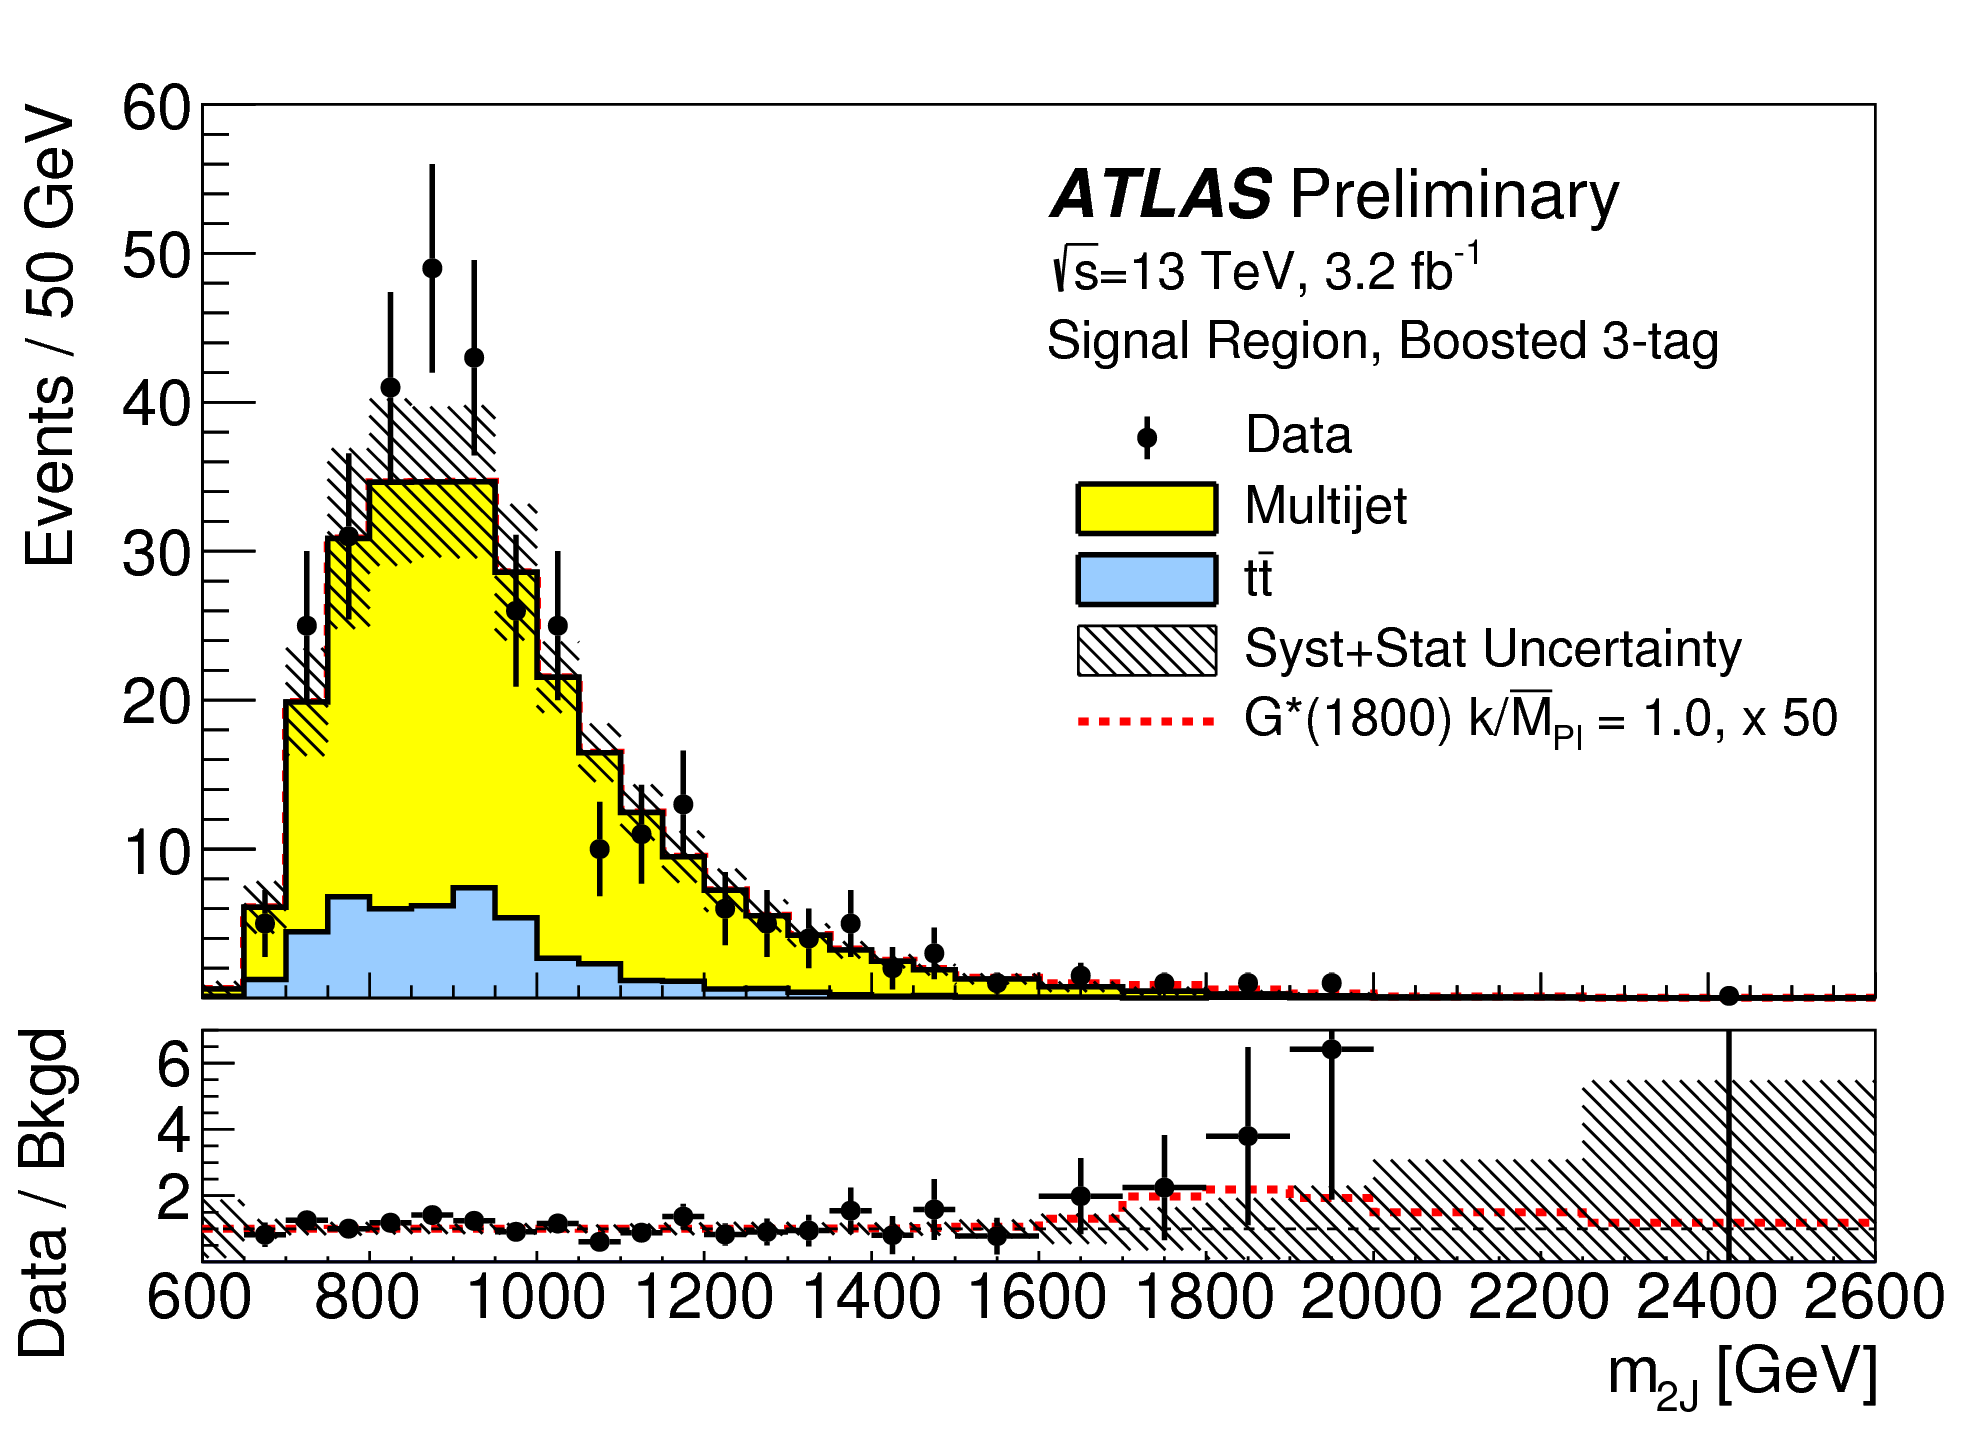
\includegraphics[width=\textwidth]{figures/3b_signal}
        \caption{}
    \end{subfigure}%
    \begin{subfigure}[t]{0.5\textwidth}
        \centering
        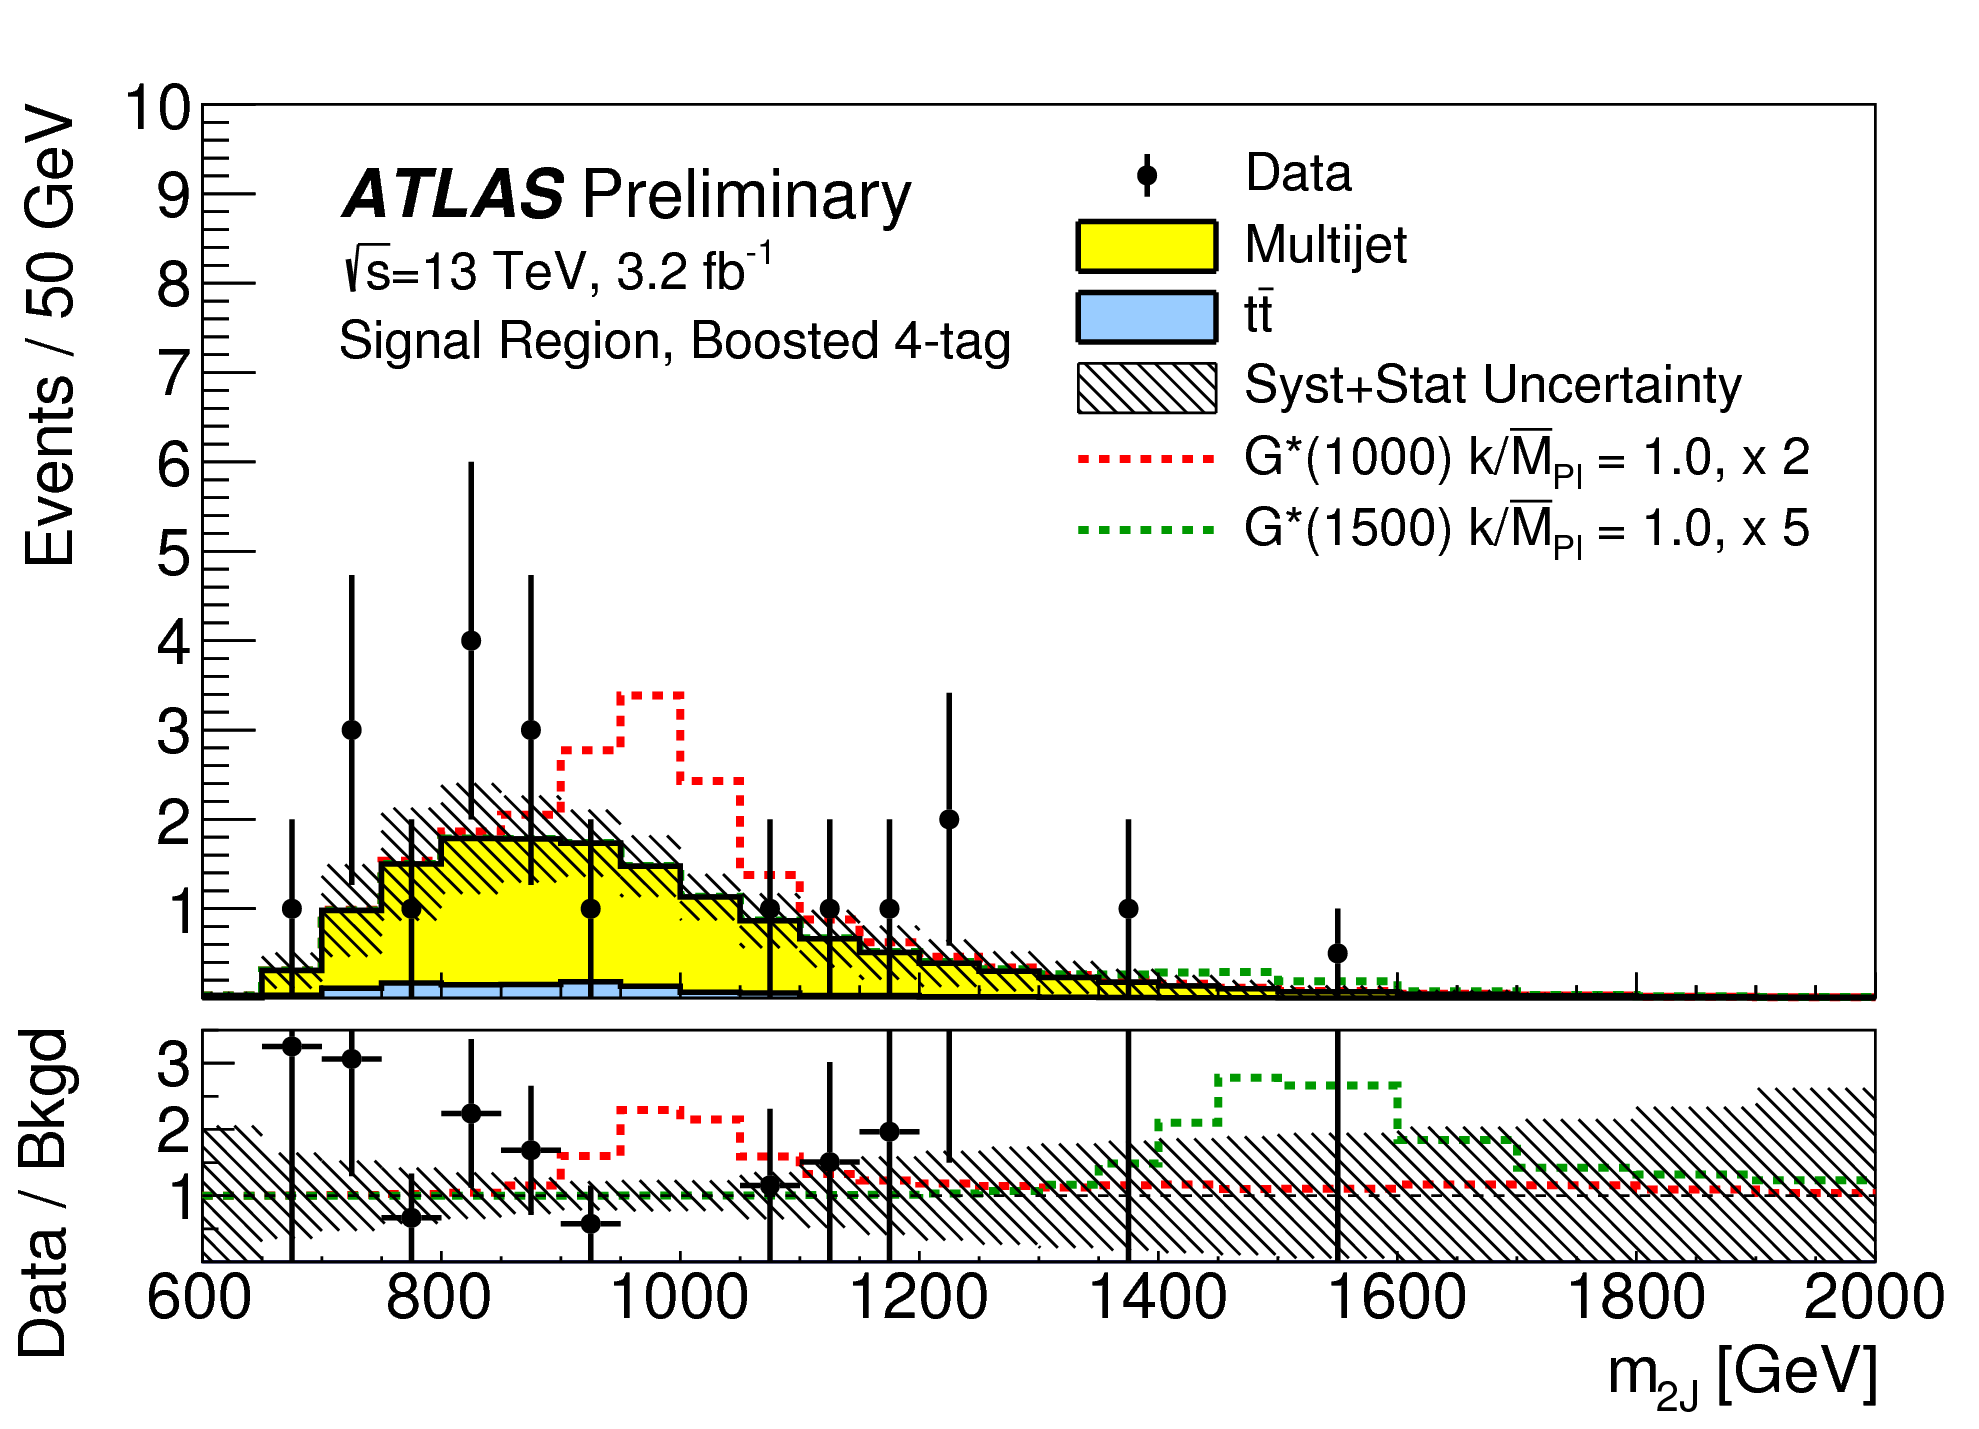
\includegraphics[width=\textwidth]{figures/4b_signal}
        \caption{}
    \end{subfigure}

   \caption{Di-jet invariant mass ($M_{2J}$) in the $3b$ (a) and $4b$ (b) signal regions. The multijet and $\ttbar$ backgrounds are estimated using the data-driven methods described above. In the $3b$ region, a graviton signal with $m_{\Gkk} = 1.8 \TeV$ and $c=1$ is overlaid, with the cross section multiplied by a factor of $50$ so that the signal is visible. In the $4b$ region, signals with $m_{\Gkk} = 1.0 \TeV$ and $m_{\Gkk} = 1.5 \TeV$ are overlaid, both with $c = 1$ and the yields multiplied by factors of $2$ and $5$ respectively~\cite{4bconf}.}
  \label{fig:BoostedResults}
\end{figure}


